\documentclass{article}
% Packages nécessaires
% knitr

% Pour les documents en francais...
	\usepackage[latin1]{inputenc}
	\usepackage[french]{babel}
	\usepackage[french]{varioref}

% Math?matiques
	\usepackage{amsmath}

% Caracteres speciaux suppl?mentaires
	\usepackage{latexsym,amsfonts}

% A documenter
	\usepackage{moreverb}

% Macros pour les paquets
	\usepackage{array}  			% N?cessaires pour les tableaux de la macro Excel.

% Outil suppl?mentaire pour les tableaux
	\usepackage{multirow}
	\usepackage{booktabs}
	\usepackage{xcolor} % alternating row colors in table, incompatible avec certains modules
	\usepackage{longtable}
	\usepackage{colortbl}

% Pour ins?rer des graphiques
	\usepackage{graphicx} 			% Graphique simples
	\usepackage{subfigure}			% Graphiques multiples

% Pour ins?rer des couleurs
	\usepackage{color}

% Rotation des objets et des pages
%	\usepackage{rotating}
%	\usepackage{lscape}

% Pour insrer du code source, LaTeX ou SAS par exemple.
	\usepackage{verbatim}
         \usepackage{moreverb}
	\usepackage{listings}
	\lstset{basicstyle=\ttfamily,
  		showstringspaces=false,
  		commentstyle=\color{red},
  		keywordstyle=\color{blue}
	}
	\usepackage{fancyvrb}

%	\lstset{language=SAS,numbers=left}		% Par dfaut le listing est en SAS

% Pour ins?rer des hyperliens
  \usepackage{hyperref}

% American Psychological Association (for bibliographic references).
	\usepackage{apacite}

% Pour l'utilisation des macros
	\usepackage{xspace}

% En têtes et pieds de pages
 	\usepackage{fancyhdr}

% Macros commandes
% Pour ins?rer des dessins de Linux
\newcommand{\LinuxA}{\includegraphics[height=0.5cm]{Graphiques/linux.png}}
\newcommand{\LinuxB}{\includegraphics[height=0.5cm]{Graphiques/linux.png}\xspace}

% Macro pour les petits dessins pour les diff?rents OS.
\newcommand{\Windows}{\emph{Windows}\xspace}
\newcommand{\Mac}{\emph{Mac OS X}\xspace}

\newcommand{\Linux}{\emph{Linux}\xspace}
\newcommand{\linux}{\emph{Linux}\xspace}

\newcommand{\GNULinux}{\emph{GNU/Linux}\xspace}
\newcommand{\gnulinux}{\emph{GNU/Linux}\xspace}

\newcommand{\Fedora}{\emph{Feodra}\xspace}
\newcommand{\Ubuntu}{\emph{Ubuntu}\xspace}


\newcommand{\MikTeX}{MiK\tex\xspace}
\newcommand{\latex}{\LaTeX\xspace}


\newcommand{\df}{\emph{data.frame}\xspace}
\newcommand{\liste}{\emph{list}\xspace}
\newcommand{\cad}{c'est-à-dire\xspace}

 % Définition de l'auteur, ...
% Titre  	 
        \title{Introduction � GNU/Linux}
        \author{Pascal Bessonneau}
				\date{11/2017}

% Pieds de page, marges, ...
% page layout

% By LaTeX commands
%\setlength{\oddsidemargin}{0cm}
%\setlength{\textwidth}{16cm}
%\setlength{\textheight}{24cm}
%\setlength{\topmargin}{-1cm}
%\setlength{\marginparsep}{0.2cm}

% fancyheader parameters
\pagestyle{fancy}  

\fancyfoot[L]{{\small Formation GNU/Linux}}
\fancyfoot[c]{} 
\fancyfoot[R]{{\small \thepage/\pageref{LastPage}}}

\fancyhead[L]{} 
\fancyhead[c]{}
\fancyhead[R]{} 

\begin{document}
\maketitle
\newpage
\tableofcontents
\newpage
\section{Rapide historique de GNU/Linux}

  \subsection{UNIX}
	
	Le premier syst�me d'exploitation a �t� con�u par  Ken Thompson et Dennis Ritchie (AT\&T Bell Laboratories)
	en 1970. Il �tait �crit en C d�j�.
	
	BSD a tent� de faire un fork mais un proc�s a eu lieu car BSD embarquait des codes propri�t�s de AT\&T.
	
	(ce qui a chang� depuis, BSD est open source compl�tement). Mais �a a frein� l'expansion de BSD.
	


  \subsection{Le noyau}
	
	Il assure l'interface entre les logiciels et le mat�riel. 
	
	MINIX, un syst�me Unix-like pour usage acad�mique a �t� �crit par Andrew S. Tanenbaum.
	
	Puis Linus Torvals, le 25 August 1991, poste un message pour dire qu'il a �crit un MINIX like en C qui 
	pouvait faire tourner un compilateur et bash (le mode console).
	
	Appel�e au d�but FreaX, il fut renommer par un administrateur d'un serveur FTP Linux. Ce qui fut accept� par Linus Torvalds.
	
	Rapidement il fut plac� sur  GNU General Public License (GPL)~: v1 puis v2 et enfin v3. 
	

	
	Il rassembla pas mal de d�veloppeurs et surtout des companies vont s'en emparer. En effet en 2015, 80\% 
	des d�veloppeurs sont r�mun�r�s pour leurs contributions.
	


  \subsection{Le projet GNU}
  
  Tout cela (le succ�s de Linux) n'aura pas eu lieu sans le projet GNU lanc� par Richard Stallman qui, 
	en 1983, a d�marr� le projet GNU  avec le projet de cr�er un clone d'UNIX opensource. La communaut� est aussi � l'origine
	des licences qui encadrent la plupart des logiciels opensource.


  \subsection{Le d�buts des distributions}
  
		En 1993 deux distributions ont �t� cr�es pour faciliter l'installation et la maintenance des syst�mes GNU/Linux~: Slackware et Debian.
		
		Aujourd'hui faire Linux from Scratch (enti�rement � la main) est reserv� � l'apprentissage. Ce sont les distributions (la pl�thore) de distributions
		qui permet d'installer et de g�rer son ordinateur sous GNU/Linux.


\section{Versions}

  \subsection{Unstable}
	
	Dans une premi�re �tape, une version exp�rimentale est r�alis�e. Elle est dite \emph{unstable}.
	
	Elle n'est pas recommand� pour les novices et en production. A ce stade les versions des logiciels ne sont pas toujours 
	fix�es.
	
	Souvent son num�ro apr�s la virgule est impaire (au moins pour les Debian et Fedora).
	

  \subsection{Release candidate}
	
	Dans cette version plus mature, la plupart des gros bugs sont r�solus. A cette �tape, les testeurs et d�veloppeurs
	chasse les derniers bugs mineures. La version des logiciels dans la distribution est fix�e � ce stade.
	
	Souvent on la voit retrouve appel�e RC pour Release Candidate, plus le nombre augmente plus la version est fiable.
			

  \subsection{Stable}
	
	Dans cette version mature, les bogues sont r�solus. A cette �tape, la distribution est stable et peut �tre install� par tous.
	
	Le temps durant lequel la communaut� fournit les mises � jour varie selon la version et la distribution (support de la version). Par exemple pour 
	la Debian c'est trois ans.
			

  \subsection{Long Term Support}
	
	Certaines distributions comme Ubuntu, distingue deux types de distributions~:
	\begin{description}
		\item les versions normales (pour Ubuntu x.10) support�es pendant une br�ve p�riode
		\item les versions LTS qui sont support�es pendant plus longtemps (pour Ubuntu x.04 pendant 5 ans)
	\end{description}
	
	

  \subsection{Trouver la version install�e}
	
	En console il suffit de taper \emph{lsb\_release -a}.
	
	Dans param�tres sous GNOME, on peut l'avoir dans le groupe \og~D�tails~\fg.
	

	
	\begin{center}
	\begin{figure}
	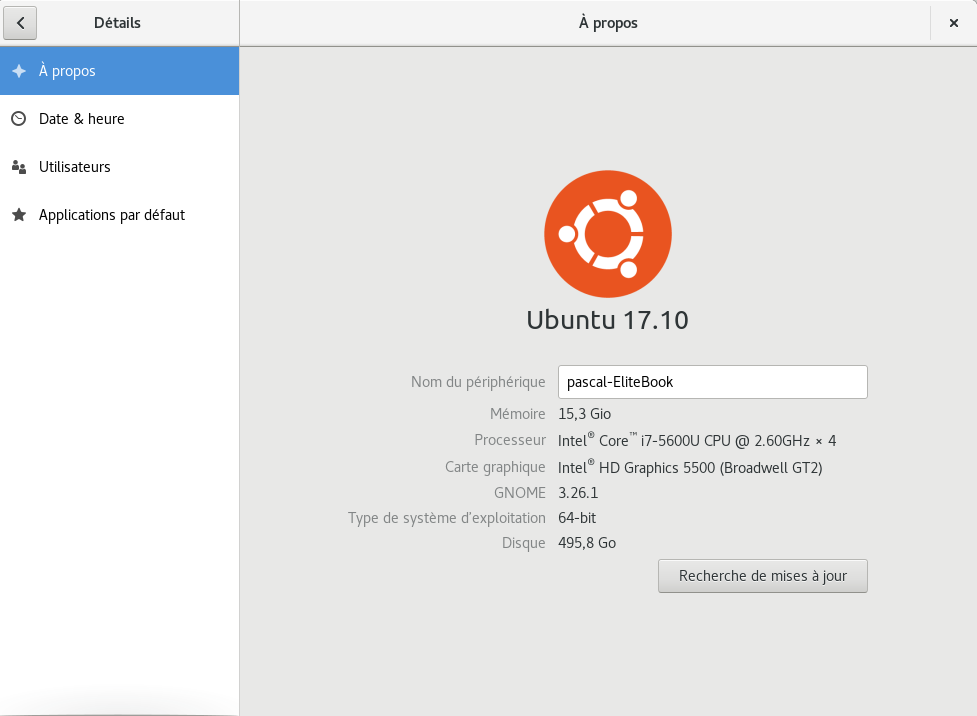
\includegraphics[scale=0.25]{Figures/Selection004}
	\caption{Version sous GNOME}
	\end{figure}
	\end{center}
	

\section{Recommandations}

  \subsection{Versions pr�conis�es}
	
	\begin{description}
		\item[Ubuntu] c'est la plus simple � utiliser pour un novice. Enfant de Debian elle a aussi le plus gros volume de documentation en ligne. Des variantes pour les ordinosaures existent comme Lubuntu
		\item[Mint] Enfant d'Ubuntu, on a les m�mes avantages mais avec un bureau par d�faut de type Cinnamon
		\item[Fedora] c'est celle, qui dans la simplicit�, vient juste apr�s. Il y a quelques manipulations � faire pour avoir les contenus
		non libres comme les plug ins Flash\dots apr�s l'installation.
		\item[Arch,Manjaro] pour les aventureux qui veulent les logiciels \og~on the edge~\fg
	\end{description}
		

  \subsection{Pr�conisations � l'installation}

	\begin{itemize}
		\item Lors de l'installation, faites la sur un disque entier puis avec ce que nous verrons, mettez le home sur un disque diff�rent pour avoir plus de place et 
	pour en cas de r�installation avoir toujours votre HOME propre.
	\end{itemize}
			

  \subsection{Pr�conisations � l'installation d'Ubuntu}

	Ubuntu installe le plugin flash, le MP3 si demand� � l'installation. Il ne reste plus grand chose � faire.
	
	A la rigueur le d�pot Google pour Chrome (Netflix, CanalPlay,\dots)~:
	
\begin{verbatim}
wget -q -O - https://dl.google.com/linux/linux_signing_key.pub | sudo apt-key add -
sudo echo "deb https://dl.google.com/linux/chrome/deb/ stable main" > /etc/apt/sources.list.d/google-chrome.list
\end{verbatim}	
			


	Et GNOME-tweak-tool si il n'est pas install�~:
\begin{verbatim}
sudo apt-get install gnome-tweak-tool	
\end{verbatim}



  \subsection{Pr�conisations � l'installation pour Fedora}

	\begin{itemize}
		\item Ajouter les d�pots rpmfusion~:
	\begin{verbatim}
sudo dnf install https://download1.rpmfusion.org/free/fedora/rpmfusion-free-release-$(rpm -E %fedora).noarch.rpm	
sudo dnf install https://download1.rpmfusion.org/nonfree/fedora/rpmfusion-nonfree-release-$(rpm -E %fedora).noarch.rpm
	\end{verbatim}
	\end{itemize}
			


	\begin{itemize}
		\item Installer Yum \emph{dnf install yum}
		\item Installer GNOME Tweak Tool \emph{dnf install gnome-tweak-tool}
		\item Installer flash-player-ppapi et/ou flash-plugin 
	\end{itemize}
	
	

	\begin{itemize}
			\item pour installer les logiciels google comme Chrome pour Netflix, \dots
\begin{verbatim}
cat << EOF > /etc/yum.repos.d/google-chrome.repo
[google-chrome]
name=google-chrome - \$basearch
baseurl=http://dl.google.com/linux/chrome/rpm/stable/\$basearch
enabled=1
gpgcheck=1
gpgkey=https://dl-ssl.google.com/linux/linux_signing_key.pub
EOF
\end{verbatim}		
		
	\end{itemize}
			









\documentclass{beamer}
\usetheme[compress]{Singapore}
%\useoutertheme{miniframes}

% \documentclass{beamer}
%\usetheme{Warsaw}

% Pour les documents en francais...
	\usepackage[latin1]{inputenc}
	\usepackage[french]{babel}
	\usepackage[french]{varioref}
%\usepackage[T1]{fontenc} 

% Math?matiques
	\usepackage{amsmath}

% Caracteres speciaux suppl?mentaires
	\usepackage{latexsym,amsfonts}

% A documenter
	\usepackage{moreverb}

% Macros pour les paquets
	\usepackage{array}  			% N?cessaires pour les tableaux de la macro Excel.

% Outil suppl?mentaire pour les tableaux
	\usepackage{multirow}
	\usepackage{booktabs}
	\usepackage{xcolor} % alternating row colors in table, incompatible avec certains modules
	\usepackage{longtable}
	\usepackage{colortbl}

% Pour ins?rer des graphiques
	\usepackage{graphicx} 			% Graphique simples
	\usepackage{subfigure}			% Graphiques multiples

% Pour ins?rer des couleurs
	\usepackage{color}

% Rotation des objets et des pages
%	\usepackage{rotating}
%	\usepackage{lscape}

% Pour insrer du code source, LaTeX ou SAS par exemple.
	\usepackage{verbatim}
         \usepackage{moreverb}
	\usepackage{listings}
	\lstset{basicstyle=\ttfamily,
  		showstringspaces=false,
  		commentstyle=\color{red},
  		keywordstyle=\color{blue}
	}
	\usepackage{fancyvrb}

%	\lstset{language=SAS,numbers=left}		% Par dfaut le listing est en SAS

% Pour ins?rer des hyperliens
  \usepackage{hyperref}

% American Psychological Association (for bibliographic references).
	\usepackage{apacite}

% Pour l'utilisation des macros
	\usepackage{xspace}

% Pour l'utilisation de notes en fin de document.
%	\usepackage{endnotes}

% Array
%	\usepackage{multirow}
%	\usepackage{booktabs}

% Rotation
%	\usepackage{rotating}

% En t?tes et pieds de pages
%	\usepackage{fancyhdr}
%	\usepackage{lastpage}


% Page layout

% By LaTeX commands
%\setlength{\oddsidemargin}{0cm}
%\setlength{\textwidth}{16cm}
%\setlength{\textheight}{24cm}
%\setlength{\topmargin}{-1cm}
%\setlength{\marginparsep}{0.2cm}

% fancyheader parameters
%\pagestyle{fancy}

%\fancyfoot[L]{{\small Formation \LaTeX, DEPP}}
%\fancyfoot[c]{}
%\fancyfoot[R]{{\small \thepage/\pageref{LastPage}}}

%\fancyhead[L]{}
%\fancyhead[c]{}
%\fancyhead[R]{}

% Pour ins?rer des dessins de Linux
\newcommand{\LinuxA}{\includegraphics[height=0.5cm]{Graphiques/linux.png}}
\newcommand{\LinuxB}{\includegraphics[height=0.5cm]{Graphiques/linux.png}\xspace}

% Macro pour les petits dessins pour les diff?rents OS.
\newcommand{\Windows}{\emph{Windows}\xspace}
\newcommand{\Mac}{\emph{Mac OS X}\xspace}

\newcommand{\Linux}{\emph{Linux}\xspace}
\newcommand{\linux}{\emph{Linux}\xspace}

\newcommand{\GNULinux}{\emph{GNU/Linux}\xspace}
\newcommand{\gnulinux}{\emph{GNU/Linux}\xspace}

\newcommand{\Fedora}{\emph{Feodra}\xspace}
\newcommand{\Ubuntu}{\emph{Ubuntu}\xspace}


\newcommand{\MikTeX}{MiK\tex\xspace}
\newcommand{\latex}{\LaTeX\xspace}


\newcommand{\df}{\emph{data.frame}\xspace}
\newcommand{\liste}{\emph{list}\xspace}
\newcommand{\cad}{c'est-�-dire\xspace}

% Titre
\title{Introduction � GNU/Linux}
\author{Pascal Bessonneau}
\institute{Starinux}
\date{11/2017}

\subtitle{S�quence de Boot}


\newcommand{\hreff}[2]{\underline{\href{#1}{#2}\xspace}}

\begin{document}

\begin{frame}
	\maketitle
\end{frame}

\begin{frame}
	\tableofcontents
\end{frame}

% Begin document %%%%%%%%%%%%%%%%%%%%%%%%%%%%%%%%%%%%%%%%%%%%%%%%%%%%%%%%%%%%%%%%%%%%%%%%%%%%%%%%%%

\section{S�quence de Boot}

\begin{frame}[containsverbatim]
  \frametitle{Recherche du software apr�s le d�marrage mat�riel}

	  Le mat�riel va chercher le software qui est n�cessaire pour booter~:
	  \begin{itemize}
	  	\item une partition bootable
	  	\item une partition \textit{UEFI}
	\end{itemize}


\end{frame}


\begin{frame}[containsverbatim]
  \frametitle{Old school}
	
	la partition doit �tre bootable. Pour la rendre bootable il suffit d'utiliser \textit{gparted} ou \textit{fdisk} pour la rendre bootable.
	
	Sinon tous les installeurs le font d'eux-m�mes.
	  
\end{frame}

\begin{frame}[containsverbatim]
  \frametitle{UEFI}
	
	L'UEFI install� sur les ordinateurs complexifie le processus en demandant que le soft de d�marrage soit sign� ce qui peut poser des probl�mes car \GNULinux.
  	
  	D'autre part il exige une partition en \text{FAT32} pour d�marrer bien particuli�re et il faut une signature particuli�re r�pondant au doux nom de \textit{EF00}. Il faut �galement que la table des partitions soit au format \textit{gpt}.
  	
  	L'\textit{UEFI} est connu pour une b�te noire pour la configuration sous \Linux. Les distributions mainstream g�rent maintenant l'\textit{UEFI}. Tant qu'on a que \Linux sur le poste. En cas de double boot, on commence � avoir des probl�mes.
  	
\end{frame}


\begin{frame}[containsverbatim]
  \frametitle{UEFI}
	
more...	
	
\end{frame}


\begin{frame}[containsverbatim]
  \frametitle{GRUB}
  
  Ensuite le d�marrage va charger en m�moire le petit noyau \linux\dots
  
  le noyau par d�faut est celui qui s'appelle vmlinuz � la racine /. En fait c'est un lien symbolique vers le noyau qui se trouve vraiment dans \textit{/boot}.
  
  \textit{GRUB} selon ses r�glages peut d�marrer sur un autre noyau. La configuration de \textit{GRUB} se fait en lan�ant \textit{update-grub}.

\end{frame}

\begin{frame}[containsverbatim]
  \frametitle{GRUB}
  
  La partie automatis�e de \textit{GRUB} est situ� dans le r�pertoire \emph{/boot/grub}. C'est l� qu'on retrouve des scripts \textit{bash} qui vont construire le menu de d�marrage et qui vont �tre appel� quand on fait \textit{update-grub}.
  
  Pour les modifications manuelles, il faut �diter le fichier \emph{40\_custom} dans \emph{/etc/grub.d} ou directement (plus simple) le fichier \emph{/etc/default/grub}.
  	
\end{frame}

\begin{frame}[containsverbatim]
  \frametitle{GRUB}
  
Point s�curit�~: il est possible avec les bons arguments de booter avec le menu \emph{d�marage personnalis�e} en mode single user, ie. en root (voir \href{https://askubuntu.com/questions/132965/how-do-i-boot-into-single-user-mode-from-grub}{ici})

Pour ne pas le permettre il faut ajouter un mot de passe � taper avant d'acc�der � cette personnalisation. 

Vous trouverez la manipulation \href{https://help.ubuntu.com/community/Grub2/Passwords}{ici}. Elle se ressemble sur \Fedora et \Ubuntu.
  	
\end{frame}

\begin{frame}[containsverbatim]
  \frametitle{vmlinuz}
  
  Il s'appelle ainsi car il est compress� � une �poque ou le programme ne devait pas d�passer une taille critique. D'ailleurs sur certains ordinateurs on �taient oblig�s de modifier (compiler soi m�me le noyau) pour qu'il rentre dans la taille sp�cifi�e.
  
  En effet il y a dans \emph{vmlinuz} le syst�me d'exploitation et et des ``modules''. Un module est un bout du noyau qui ajoute des fonctionnalit�s~: une interface pour un mat�riel particulier, la possibilit� de lire un format de fichier, \dots
  	
\end{frame}

\begin{frame}[containsverbatim]
  \frametitle{vmlinuz}
  
  Au d�marrage dans \emph{GRUB}, on peut charger un module ou au contraire emp�cher son chargement. 
  
  C'est utile par exemple � l'heure o� j'�cris ces lignes pour une installation avec la carte Nvidia pour \Fedora (pareil sous \Ubuntu) \href{ https://www.if-not-true-then-false.com/2015/fedora-nvidia-guide/}{ici}.
  
  Le principe des modules est qu'ils sont charg�s � la demande du noyau et �vite ainsi d'avoir un noyau �norme et qui serait moins performant (?).
  
\end{frame}


\begin{frame}[containsverbatim]
  \frametitle{init/system.d}
  
  A ce stade, nous sommes en pleine transition en deux logiciels pour continuer le d�marrage, le syst�me \emph{init} et le \emph{systemd}.
  
 Le syst�me \emph{init} est en phase d'�tre abandonn� au profit de l'autre. 
 
 Dans la plupart des distributions vous pouvez constater leur travail en appuyant sur la touche \emph{ESC} de votre ordinateur. Vous verrez une ligne par service charg�.
 
 Par service, il faut entendre qu'il va charger le support r�seau, le support du mat�riel, \dots

\end{frame}


\begin{frame}[containsverbatim]
  \frametitle{init/systemd}
  
  Sous \Fedora le systemd est presque compl�tement adopt�. Sous Ubuntu c'est moins clair car ils ont essay� de lancer leur propre syst�me de d�marrage \emph{Upstart} qui n'a pas pris dans la communaut�. Donc Ubuntu c'est un peu le f...
  
  Pour activer ou d�sactiver un service de systemd, il faut utiliser la commande \emph{sysctl}.
  
  Vous pouvez regarder \href{https://wiki.debian.org/fr/systemd}{l�}. 
  
  Les diff�rents services sont th�oriquement dans le r�pertoire \emph{/etc/systemd/system}.
  
\end{frame}

\begin{frame}[containsverbatim]
  \frametitle{run.level}
  
  Pour g�rer un service init, c'est les commandes~:
  \begin{verbatim}
  update-rc.d <nom du service> stop|start|enable|disable
  \end{verbatim}
  
  Il faut parfois rajouter l'option \emph{-f} pour pour forcer la commande. Il vous le signale si c'est n�cessaire.
  
\end{frame}

\begin{frame}[containsverbatim]
  \frametitle{run.level}
  
  Les \emph{run.levels} sont fondamental dans \Linux. Ils sont appel�s aussi par l'appellation System V.
  
  Une machine \Linux est toujours dans un �tat d�fini par un \emph{run.level}. Par exemple le mode multi-user (g�n�ralement \emph{rc2.d}), il a un \emph{run.level} \emph{rc0} pour l'extinction, le single user le \emph{rcS}\dots
  
  Ces �tats sont d�crits dans un fichier particulier \emph{/etc/inittab}.
  
\end{frame}

\begin{frame}[containsverbatim]
  \frametitle{Interface de connexion graphique}
  
	L'interface de connexion graphique est maintenant lanc� par d�faut pour la plupart des \GNULinux. 
	
	Cette interface vous permet de vous authentifier et de lancer votre  bureau pr�f�r�. 
	
	Une interface a �t� cr��e par la plupart des bureaux mais vous avez avoir une interface GNOME et lancer KDE.
  
  
\end{frame}

\begin{frame}[containsverbatim]
  \frametitle{Interface de connexion graphique}
  
	Les plus connues sont �videmment celles des bureaux les plus connus~: \emph{kdm} (KDE), \emph{gdm} (GNOME), \emph{lightdm} (LXDE),\dots
	
  La m�thode la plus simple pour reconfigurer l'interface de d�marrage (passer de l'une � l'autre) est de lancer la configuration de l'interface install�e~:
	\begin{verbatim}
dpkg-reconfigure gdm	
	\end{verbatim}
  
\end{frame}

\begin{frame}[containsverbatim]
  \frametitle{Xorg, Wayland}
  
	Xorg est une couche logicielle qui permet d'avoir des interfaces graphiques sous \GNULinux. 
	
	Il provient d'une anc�tre qui s'appellait X sous UNIX. Il est en passe d'�tre remplacer dans les prochains mois par Wayland. C'est d�j� le cas sous Fedora.
  
	C'est la couche qui va g�rer votre �cran, votre souris, \dots Il est � l'interface entre le bureau et le mat�riel.
		
\end{frame}


\begin{frame}[containsverbatim]
  \frametitle{Bureau}
	
	Le bureau est sch�matiquement un gestionnaire de fen�tre avec des applications d�di�es.
	
	Les plus connus sont GNOME, KDE, Mate, Cinnamon, \dots
  
	  
\end{frame}

\begin{frame}[containsverbatim]
  \frametitle{En cas de probl�me lors du d�marrage}
	
	Si votre ordinateur sous \GNULinux ne d�marre pas, il existe des solutions plus ou moins simples pour savoir ce qui cloche~:
	\begin{enumerate}
		\item Si le menu GRUB ne s'affiche pas c'est que le boot ou l'UEFI ne marche pas
		\item Si \Windows se lance au lieu de \GNULinux c'est que le boot ou l'UEFI ne marche pas
		\item Si en appuyant sur \emph{ESC} vous voyez que l'ordinateur bloque sur un service, c'est peut �tre ce service
		\item Si l'ordinateur s'arr�te et demande � passer en root pour des r�parations, un service ou un p�riph�rique (ex~: disque dur manquant) ne fonctionne pas
	\end{enumerate}
	  
\end{frame}


\begin{frame}[containsverbatim]
  \frametitle{En cas de probl�me lors du d�marrage}
	
	\begin{enumerate}
		\item Si l'ordinateur reste noir ou bloqu� sur l'�cran de d�marrage, vous pouvez essayer de voir si la console est disponible sur les autres terminals (CTRL+ALT+F1, CTRL+ALT+F2,\dots). Si une console est disponible, alors c'est l'interface de d�marrage graphique qui bloque ou Xorg.
		\item Si l'ordinateur revient � l'interface graphique de connexion par exemple c'est le bureau qui est en cause ou votre \emph{home} directory (le bureau ne d�marre pas si votre home n'est pas accessible en lecture ou s'il est plein).
	\end{enumerate}
	  
\end{frame}

\begin{frame}[containsverbatim]
  \frametitle{Pour conna�tre la version du gestionnaire de fen�tres}

	La commande la plus efficace est surement la commande~:
\begin{verbatim}
printf 'Desktop: %s\nSession: %s\n' "$XDG_CURRENT_DESKTOP" "$GDMSESSION"
\end{verbatim}
\end{frame}

\end{document}




\documentclass{beamer}
\usetheme[compress]{Singapore}
%\useoutertheme{miniframes}

% \documentclass{beamer}
%\usetheme{Warsaw}

% Pour les documents en francais...
	\usepackage[latin1]{inputenc}
	\usepackage[french]{babel}
	\usepackage[french]{varioref}
%\usepackage[T1]{fontenc} 

% Math?matiques
	\usepackage{amsmath}

% Caracteres speciaux suppl?mentaires
	\usepackage{latexsym,amsfonts}

% A documenter
	\usepackage{moreverb}

% Macros pour les paquets
	\usepackage{array}  			% N?cessaires pour les tableaux de la macro Excel.

% Outil suppl?mentaire pour les tableaux
	\usepackage{multirow}
	\usepackage{booktabs}
	\usepackage{xcolor} % alternating row colors in table, incompatible avec certains modules
	\usepackage{longtable}
	\usepackage{colortbl}

% Pour ins?rer des graphiques
	\usepackage{graphicx} 			% Graphique simples
	\usepackage{subfigure}			% Graphiques multiples

% Pour ins?rer des couleurs
	\usepackage{color}

% Rotation des objets et des pages
%	\usepackage{rotating}
%	\usepackage{lscape}

% Pour insrer du code source, LaTeX ou SAS par exemple.
	\usepackage{verbatim}
         \usepackage{moreverb}
	\usepackage{listings}
	\lstset{basicstyle=\ttfamily,
  		showstringspaces=false,
  		commentstyle=\color{red},
  		keywordstyle=\color{blue}
	}
	\usepackage{fancyvrb}

%	\lstset{language=SAS,numbers=left}		% Par dfaut le listing est en SAS

% Pour ins?rer des hyperliens
  \usepackage{hyperref}

% American Psychological Association (for bibliographic references).
	\usepackage{apacite}

% Pour l'utilisation des macros
	\usepackage{xspace}

% Pour l'utilisation de notes en fin de document.
%	\usepackage{endnotes}

% Array
%	\usepackage{multirow}
%	\usepackage{booktabs}

% Rotation
%	\usepackage{rotating}

% En t?tes et pieds de pages
%	\usepackage{fancyhdr}
%	\usepackage{lastpage}


% Page layout

% By LaTeX commands
%\setlength{\oddsidemargin}{0cm}
%\setlength{\textwidth}{16cm}
%\setlength{\textheight}{24cm}
%\setlength{\topmargin}{-1cm}
%\setlength{\marginparsep}{0.2cm}

% fancyheader parameters
%\pagestyle{fancy}

%\fancyfoot[L]{{\small Formation \LaTeX, DEPP}}
%\fancyfoot[c]{}
%\fancyfoot[R]{{\small \thepage/\pageref{LastPage}}}

%\fancyhead[L]{}
%\fancyhead[c]{}
%\fancyhead[R]{}

% Pour ins?rer des dessins de Linux
\newcommand{\LinuxA}{\includegraphics[height=0.5cm]{Graphiques/linux.png}}
\newcommand{\LinuxB}{\includegraphics[height=0.5cm]{Graphiques/linux.png}\xspace}

% Macro pour les petits dessins pour les diff?rents OS.
\newcommand{\Windows}{\emph{Windows}\xspace}
\newcommand{\Mac}{\emph{Mac OS X}\xspace}

\newcommand{\Linux}{\emph{Linux}\xspace}
\newcommand{\linux}{\emph{Linux}\xspace}

\newcommand{\GNULinux}{\emph{GNU/Linux}\xspace}
\newcommand{\gnulinux}{\emph{GNU/Linux}\xspace}

\newcommand{\Fedora}{\emph{Feodra}\xspace}
\newcommand{\Ubuntu}{\emph{Ubuntu}\xspace}


\newcommand{\MikTeX}{MiK\tex\xspace}
\newcommand{\latex}{\LaTeX\xspace}


\newcommand{\df}{\emph{data.frame}\xspace}
\newcommand{\liste}{\emph{list}\xspace}
\newcommand{\cad}{c'est-�-dire\xspace}

% Titre
\title{Introduction � GNU/Linux}
\author{Pascal Bessonneau}
\institute{Starinux}
\date{11/2017}

\subtitle{Travailler en mode console}


\newcommand{\hreff}[2]{\underline{\href{#1}{#2}\xspace}}

\begin{document}

\begin{frame}
	\maketitle
\end{frame}

\begin{frame}
	\tableofcontents
\end{frame}

% Begin document %%%%%%%%%%%%%%%%%%%%%%%%%%%%%%%%%%%%%%%%%%%%%%%%%%%%%%%%%%%%%%%%%%%%%%%%%%%%%%%%%%

\section{Acc�der au terminal}

\subsection{Introduction}

\begin{frame}[containsverbatim]
  \frametitle{Terminal/Console}

	Le Terminal est souvent n�cessaire sous \Linux. Plus pr�cisement il est souvent plus facile de passer
	par le Terminal pour faire des r�glages qu'en mode graphique.
	
	C'est � la fois un plus et le talon d'Achille de \Linux.
		
\end{frame}

\begin{frame}[containsverbatim]
  \frametitle{Terminal/Console}

	Le Terminal est souvent dans le r�pertoire des outils syst�mes (KDE, Cinnamon,\dots). Il s'appelle \emph{Terminal} dans Gnome3. 
	
	On peut le lancer et ouvrir plusieurs sessions (les logiciels supportent quasiment tous plusieurs
	sessions). Chaque session �tant ind�pendante.
	
	La console est aussi accessible sur les bureaux CTRL+ALT+F1, CTRL+ALT+F2, \dots,  CTRL+ALT+F5.	Initialement l'interface graphique �tait sur le bureau 6 ou 7 maintenant on peux le trouver sur le bureau 1 ou 2.
	
\end{frame}

\section{Commandes primaires}

\begin{frame}[containsverbatim]
  \frametitle{Raccourcis clavier}

	Vous pouvez utiliser la fl�che haute pour rappeler des commandes d�j� soumises.
	\vspace{1em}
	Si vous tapez le d�but d'une commande ou d'un fichier vous pouvez compl�ter avec Tab.
		
\end{frame}

\begin{frame}[containsverbatim]
  \frametitle{Terminal/Console}

	Les commandes primaires seront~:
	\begin{description}
		\item[cd] change de r�pertoire. Pour changer de r�pertoire il suffit de donner son nom, vide vous retournez � votre r�pertoire personnel.
		\item[ls] liste les fichiers et r�pertoires. Pour avoir les d�tails sur les fichiers utiliser \emph{ls -l}
		\item[cp] copie les fichiers et r�pertoires. 
		\item[mv] copie les fichiers et r�pertoires. 
		\item[pwd] affiche le r�pertoire courant (actif)
		\item[nano] �diteur de texte. il suffit d'ajouter le nom du fichier � ouvrir
	\end{description}
	
\end{frame}

\begin{frame}[containsverbatim]
  \frametitle{cd}
		
		\begin{description}
			\item[cd] retourne au r�pertoire personnel
			\item[cd ..] va au r�pertoire parent
			\item[cd items/sauvegarde] va dans le r�pertoire items/sauvegarde
			\item[cd /var/items/sauvegarde] va dans le r�pertoire /var/items/sauvegarde
			\item[cd \textasciitilde pascal] va dans le r�pertoire personnel de pascal
		\end{description}
	
\end{frame}

\begin{frame}[containsverbatim]
  \frametitle{ls}
		
		\begin{description}
			\item[ls] liste les fichiers
			\item[ls -l] liste les fichiers avec les d�tails
			\item[ls -la] liste les fichiers avec les d�tails y compris les fichiers cach�s
		\end{description}
	
\end{frame}

\begin{frame}[containsverbatim]
  \frametitle{cp}
		
		\begin{description}
			\item[cp a b] copie le fichier a en b
			\item[cp -f a b] �crase le fichier b avec le contenu du fichier a
			\item[cp -R d e] copie tout le r�pertoire d dans le r�pertoire e
		\end{description}
	
\end{frame}

\begin{frame}[containsverbatim]
  \frametitle{mv}
		
		\begin{description}
			\item[mv a b] d�place le fichier a en b
			\item[mv -f a b] d�place en �crasant le fichier b avec le contenu du fichier a
			\item[mv -R d e] d�place tout le r�pertoire en r�pertoire e
		\end{description}
	
\end{frame}

\begin{frame}[containsverbatim]
  \frametitle{pwd}
		
		Pour p(ath) w(orking) d(irectory), cette commande affiche le r�pertoire courant ou actif.
		
		
\end{frame}

\section{Utilitaires pour le texte}


\begin{frame}[containsverbatim]
  \frametitle{Copier/Coller dans un Terminal}
		
		Pour copier un texte depuis la console, il faut utiliser la commande \emph{CTRL+INS} et pour 
		coller dans la console, il faut utiliser la commande \emph{SHIFT+INS}. 
		
\end{frame}


\begin{frame}[containsverbatim]
  \frametitle{nano}
		
		\begin{description}
			\item[nano fichier] ouvre le fichier fichier
		\end{description}

			\begin{itemize}
    \item Pour �crire dans un fichier ou le sauvegarder, utilisez Ctrl-o
    \item Pour quitter Nano, Ctrl-x
    \item Pour rechercher dans le fichier, Ctrl-w
\end{itemize}
	
\end{frame}

\begin{frame}[containsverbatim]
  \frametitle{nano}
		
		Pour le copier/coller, il faut au d�but du texte � copier faire CTRL-shift-6, puis fl�che gauche/droite pour s�lectionner le texte.
		
		La s�lection finie il faut appuyer sur Alt-Shift-6.
		
		Pour le coller, il faut appuyer sur CTRL-u.
				
\end{frame}

\begin{frame}[containsverbatim]
  \frametitle{nano}
		
		Pour l'affichage de fichiers texte comme les logs il y a 4 commandes � se rappeler~:
		
		\begin{itemize}
			\item[head -<n>] affiche les n premi�res lignes d'un fichier
			\item[tail -<n>] affiche les n premi�res lignes d'un fichier
			\item[cat] affiche tout le fichier dans la console du haut vers le bas
			\item[tac] affiche tout le fichier dans la console du bas vers le haut
		\end{itemize}
				
\end{frame}

\begin{frame}[containsverbatim]
  \frametitle{more}
		
		Pour l'affichage de grands fichiers texte~: \emph{more} ou \emph{less} affiche le fichier 
		page par page (espace pour changer de page et q pour quitter)
				
\end{frame}

\section{le \emph{PATH}}
\begin{frame}[containsverbatim]
  \frametitle{Notion}
		
		Le \emph{PATH} est l'ordre et les r�pertoires dans lequels le syst�me va chercher 
		les fichiers ex�cutables.
		
		On peut le visualiser en tapant la commande \emph{echo $PATH}.
		 
		 Le syst�me va d'abord chercher les ex�cutables dans le \emph{PATH} dans l'ordre 
		 donn� par l'ordre des r�pertoires dans le \emph{PATH}.
		 
		 Le r�pertoire courant est utilis� si l'ex�cutable n'est pas trouv� dans le \emph{PATH}.
		 		
\end{frame}

\begin{frame}[containsverbatim]
  \frametitle{Appel d'un ex�cutable}
		
		Ainsi si on �crit un ex�cutable \emph{more} et on qu'on essaie de l'appeler alors qu'il 
		est dans le r�pertoire courant, le syst�me va pr�f�rer le \emph{more} pr�sent dans \emph{/bin}.
		
		Pour lancer l'ex�cutable du r�pertoire courant, il faut l'appeler par la commande \emph{./more}.
		
		A noter que ce n'est pas recommand� de donner le nom � un ex�cutable d'un programme ex�cutable.
		
		Pour savoir quel est le r�pertoire d'un ex�cutable dans le \emph{PATH} 
		il faut utiliser la commande \emph{which}.
		
		 		
\end{frame}

\begin{frame}[containsverbatim]
  \frametitle{Trouver le r�pertoire d'une commande syst�me}
		
		Pour savoir quel est le r�pertoire d'un ex�cutable dans le \emph{PATH} 
		il faut utiliser la commande \emph{which}.
\begin{verbatim}
pascal@pascal-ordi:~$ which more
/bin/more
\end{verbatim}
		 		
\end{frame}


\end{document}
\documentclass{beamer}
\usetheme[compress]{Singapore}
%\useoutertheme{miniframes}

% \documentclass{beamer}
%\usetheme{Warsaw}

% Pour les documents en francais...
	\usepackage[latin1]{inputenc}
	\usepackage[french]{babel}
	\usepackage[french]{varioref}
%\usepackage[T1]{fontenc} 

% Math?matiques
	\usepackage{amsmath}

% Caracteres speciaux suppl?mentaires
	\usepackage{latexsym,amsfonts}

% A documenter
	\usepackage{moreverb}

% Macros pour les paquets
	\usepackage{array}  			% N?cessaires pour les tableaux de la macro Excel.

% Outil suppl?mentaire pour les tableaux
	\usepackage{multirow}
	\usepackage{booktabs}
	\usepackage{xcolor} % alternating row colors in table, incompatible avec certains modules
	\usepackage{longtable}
	\usepackage{colortbl}

% Pour ins?rer des graphiques
	\usepackage{graphicx} 			% Graphique simples
	\usepackage{subfigure}			% Graphiques multiples

% Pour ins?rer des couleurs
	\usepackage{color}

% Rotation des objets et des pages
%	\usepackage{rotating}
%	\usepackage{lscape}

% Pour insrer du code source, LaTeX ou SAS par exemple.
	\usepackage{verbatim}
         \usepackage{moreverb}
	\usepackage{listings}
	\lstset{basicstyle=\ttfamily,
  		showstringspaces=false,
  		commentstyle=\color{red},
  		keywordstyle=\color{blue}
	}
	\usepackage{fancyvrb}

%	\lstset{language=SAS,numbers=left}		% Par dfaut le listing est en SAS

% Pour ins?rer des hyperliens
  \usepackage{hyperref}

% American Psychological Association (for bibliographic references).
	\usepackage{apacite}

% Pour l'utilisation des macros
	\usepackage{xspace}

% Pour l'utilisation de notes en fin de document.
%	\usepackage{endnotes}

% Array
%	\usepackage{multirow}
%	\usepackage{booktabs}

% Rotation
%	\usepackage{rotating}

% En t?tes et pieds de pages
%	\usepackage{fancyhdr}
%	\usepackage{lastpage}


% Page layout

% By LaTeX commands
%\setlength{\oddsidemargin}{0cm}
%\setlength{\textwidth}{16cm}
%\setlength{\textheight}{24cm}
%\setlength{\topmargin}{-1cm}
%\setlength{\marginparsep}{0.2cm}

% fancyheader parameters
%\pagestyle{fancy}

%\fancyfoot[L]{{\small Formation \LaTeX, DEPP}}
%\fancyfoot[c]{}
%\fancyfoot[R]{{\small \thepage/\pageref{LastPage}}}

%\fancyhead[L]{}
%\fancyhead[c]{}
%\fancyhead[R]{}

% Pour ins?rer des dessins de Linux
\newcommand{\LinuxA}{\includegraphics[height=0.5cm]{Graphiques/linux.png}}
\newcommand{\LinuxB}{\includegraphics[height=0.5cm]{Graphiques/linux.png}\xspace}

% Macro pour les petits dessins pour les diff?rents OS.
\newcommand{\Windows}{\emph{Windows}\xspace}
\newcommand{\Mac}{\emph{Mac OS X}\xspace}

\newcommand{\Linux}{\emph{Linux}\xspace}
\newcommand{\linux}{\emph{Linux}\xspace}

\newcommand{\GNULinux}{\emph{GNU/Linux}\xspace}
\newcommand{\gnulinux}{\emph{GNU/Linux}\xspace}

\newcommand{\Fedora}{\emph{Feodra}\xspace}
\newcommand{\Ubuntu}{\emph{Ubuntu}\xspace}


\newcommand{\MikTeX}{MiK\tex\xspace}
\newcommand{\latex}{\LaTeX\xspace}


\newcommand{\df}{\emph{data.frame}\xspace}
\newcommand{\liste}{\emph{list}\xspace}
\newcommand{\cad}{c'est-�-dire\xspace}

% Titre
\title{Introduction � GNU/Linux}
\author{Pascal Bessonneau}
\institute{Starinux}
\date{11/2017}

\subtitle{Utilisateurs}


\newcommand{\hreff}[2]{\underline{\href{#1}{#2}\xspace}}

\begin{document}

\begin{frame}
	\maketitle
\end{frame}

\begin{frame}
	\tableofcontents
\end{frame}

% Begin document %%%%%%%%%%%%%%%%%%%%%%%%%%%%%%%%%%%%%%%%%%%%%%%%%%%%%%%%%%%%%%%%%%%%%%%%%%%%%%%%%%

\section{Introduction}

\begin{frame}[containsverbatim]
  \frametitle{Qu'est ce qu'un utilisateur ?}
	
	C'est un compte permettant g�n�ralement une connexion (graphique ou console).
	
	Il est associ� sous UNIX � un num�ro qui est utilis� pour identifier les fichier et les r�pertoires
	
	Il est g�n�ralement associ� � la pr�sence d'un r�pertoire utilisateur qui lui appartient.

\end{frame}

\begin{frame}[containsverbatim]
  \frametitle{Qu'est ce qu'un utilisateur ?}

	Il existe des utilisateurs sp�ciaux qui n'ont pas de r�pertoire et/ou la connexion n'est pas possible.
	
	C'est le cas pour de nombreux serveurs qui fonctionnent ainsi pour des raisons de s�curit�.
	
\end{frame}

\section{Gestion des utilisateurs}

\begin{frame}[containsverbatim]
  \frametitle{Cr�er/supprimer un utilisateur}

	Pour cr�er un utilisateur, il suffit d'utiliser la commande \emph{adduser <utilisateur>} pr�c�d� de \emph{sudo}.
	
	Et apr�s il faut r�pondre aux questions, relativement simple.
	
	En effet la gestion des utilisateurs est r�serv� au super utilisateur.

	Pour supprimer un utilisateur, il faut utiliser \emph{deluser <utilisateur>} et de r�pondre aux questions.
		
\end{frame}

\begin{frame}[containsverbatim]
  \frametitle{Les fichiers de r�f�rence}
	
	Le fichier des utilisateurs est le fichier /etc/passwd.
	
	Le fichier des groupes est le fichier /etc/group.
	
	Le fichier des groupes est plus int�ressant car il permet de voir quels groupes contiennent quels utilisateurs.
	C'est utile par exemple pour copier les droits de l'utilisateur cr�� par d�faut par votre distribution.

	\textcolor{red}{Mais il faut �viter de manipuler directement ces fichiers car s'ils sont corrompus le syst�me d'authentification peut planter}
\end{frame}

\begin{frame}[containsverbatim]
  \frametitle{Gestion des groupes}
	
	Pour ajouter un groupe � un utilisateur, il faut utiliser la commande~:
	\emph{usermod -a -G <groupe> <utilisateur>}.
	
	Pour ajouter un groupe � un utilisateur, il faut utiliser la commande~:
	\emph{gpasswd -d <utilisateur> <group>}.
		
\end{frame}

\begin{frame}[containsverbatim]
  \frametitle{Nota bene}
	
	Les droits sont des num�ros.
	
	Si l'utilisateur pascal est 1001 sur un ordinateur et 1002 sur un autre ordinateur, alors
	si vous �changez les disques les fichiers ne seront pas reconnus comme pascal sur l'un
	ou l'autre des ordinateurs.
		
\end{frame}

\begin{frame}[containsverbatim]
  \frametitle{En mode graphique}
	
	Sous KDE, l'utilitaire KUser permet de le faire graphiquement comme system-config-users sous GNOME.
		
\end{frame}

\begin{frame}[containsverbatim]
  \frametitle{Sous GNOME 3}

\begin{center}
\begin{figure}
 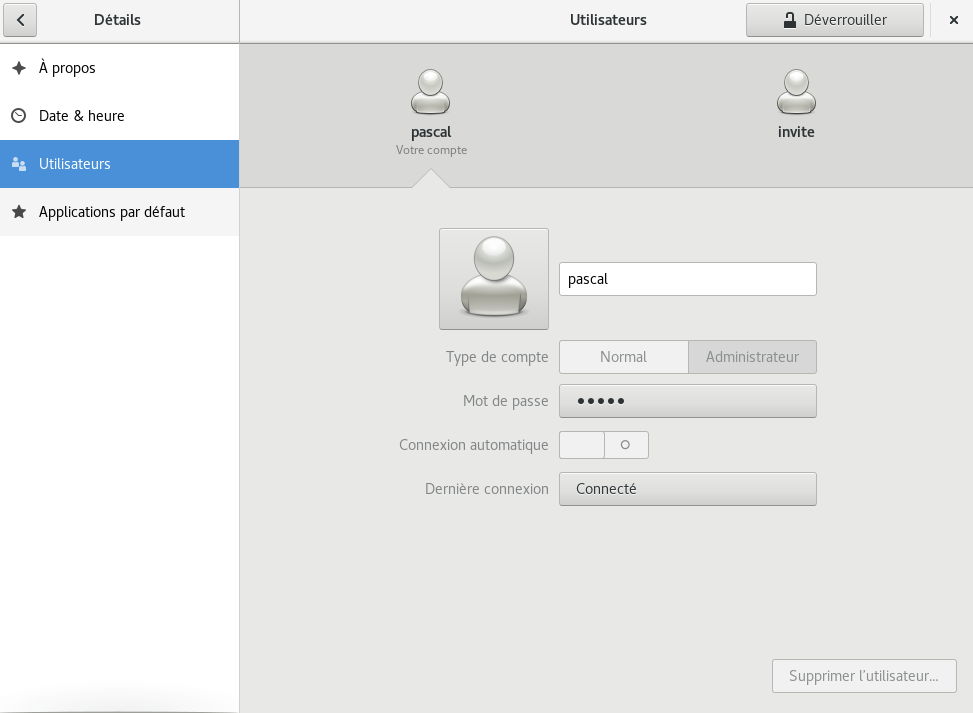
\includegraphics[scale=0.2]{Figures/Selection005}
	\caption{Utilisateurs dans le menu D�tails de l'application Param�tres}
\end{figure}
\end{center}
  
  \end{frame}

\begin{frame}[containsverbatim]
  \frametitle{Sous GNOME 3}

\begin{center}
\begin{figure}
 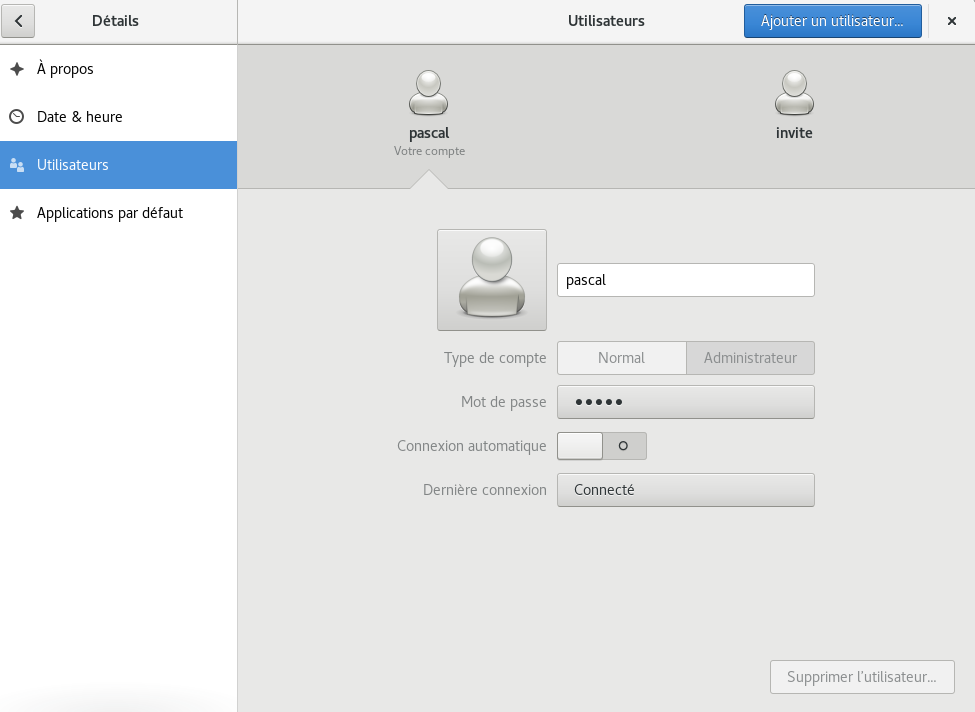
\includegraphics[scale=0.2]{Figures/Selection006}
	\caption{Utilisateurs, d�blocage avec le mot de passe}
\end{figure}
\end{center}
  
  \end{frame}


\begin{frame}[containsverbatim]
  \frametitle{Sous GNOME 3}

\begin{center}
\begin{figure}
 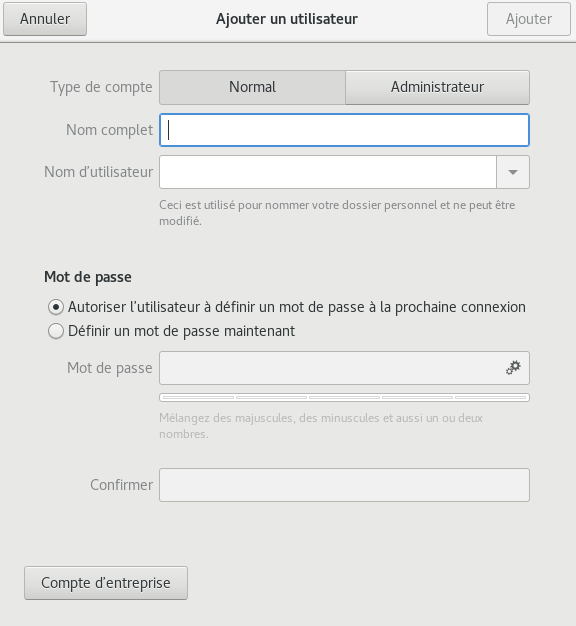
\includegraphics[scale=0.2]{Figures/Selection007}
	\caption{Utilisateurs, nouvel utilisateur}
\end{figure}
\end{center}
  
  \end{frame}

	
\end{document}
\documentclass{beamer}
\usetheme[compress]{Singapore}
%\useoutertheme{miniframes}

% \documentclass{beamer}
%\usetheme{Warsaw}

% Pour les documents en francais...
	\usepackage[latin1]{inputenc}
	\usepackage[french]{babel}
	\usepackage[french]{varioref}
%\usepackage[T1]{fontenc} 

% Math?matiques
	\usepackage{amsmath}

% Caracteres speciaux suppl?mentaires
	\usepackage{latexsym,amsfonts}

% A documenter
	\usepackage{moreverb}

% Macros pour les paquets
	\usepackage{array}  			% N?cessaires pour les tableaux de la macro Excel.

% Outil suppl?mentaire pour les tableaux
	\usepackage{multirow}
	\usepackage{booktabs}
	\usepackage{xcolor} % alternating row colors in table, incompatible avec certains modules
	\usepackage{longtable}
	\usepackage{colortbl}

% Pour ins?rer des graphiques
	\usepackage{graphicx} 			% Graphique simples
	\usepackage{subfigure}			% Graphiques multiples

% Pour ins?rer des couleurs
	\usepackage{color}

% Rotation des objets et des pages
%	\usepackage{rotating}
%	\usepackage{lscape}

% Pour insrer du code source, LaTeX ou SAS par exemple.
	\usepackage{verbatim}
         \usepackage{moreverb}
	\usepackage{listings}
	\lstset{basicstyle=\ttfamily,
  		showstringspaces=false,
  		commentstyle=\color{red},
  		keywordstyle=\color{blue}
	}
	\usepackage{fancyvrb}

%	\lstset{language=SAS,numbers=left}		% Par dfaut le listing est en SAS

% Pour ins?rer des hyperliens
  \usepackage{hyperref}

% American Psychological Association (for bibliographic references).
	\usepackage{apacite}

% Pour l'utilisation des macros
	\usepackage{xspace}

% Pour l'utilisation de notes en fin de document.
%	\usepackage{endnotes}

% Array
%	\usepackage{multirow}
%	\usepackage{booktabs}

% Rotation
%	\usepackage{rotating}

% En t?tes et pieds de pages
%	\usepackage{fancyhdr}
%	\usepackage{lastpage}


% Page layout

% By LaTeX commands
%\setlength{\oddsidemargin}{0cm}
%\setlength{\textwidth}{16cm}
%\setlength{\textheight}{24cm}
%\setlength{\topmargin}{-1cm}
%\setlength{\marginparsep}{0.2cm}

% fancyheader parameters
%\pagestyle{fancy}

%\fancyfoot[L]{{\small Formation \LaTeX, DEPP}}
%\fancyfoot[c]{}
%\fancyfoot[R]{{\small \thepage/\pageref{LastPage}}}

%\fancyhead[L]{}
%\fancyhead[c]{}
%\fancyhead[R]{}

% Pour ins?rer des dessins de Linux
\newcommand{\LinuxA}{\includegraphics[height=0.5cm]{Graphiques/linux.png}}
\newcommand{\LinuxB}{\includegraphics[height=0.5cm]{Graphiques/linux.png}\xspace}

% Macro pour les petits dessins pour les diff?rents OS.
\newcommand{\Windows}{\emph{Windows}\xspace}
\newcommand{\Mac}{\emph{Mac OS X}\xspace}

\newcommand{\Linux}{\emph{Linux}\xspace}
\newcommand{\linux}{\emph{Linux}\xspace}

\newcommand{\GNULinux}{\emph{GNU/Linux}\xspace}
\newcommand{\gnulinux}{\emph{GNU/Linux}\xspace}

\newcommand{\Fedora}{\emph{Feodra}\xspace}
\newcommand{\Ubuntu}{\emph{Ubuntu}\xspace}


\newcommand{\MikTeX}{MiK\tex\xspace}
\newcommand{\latex}{\LaTeX\xspace}


\newcommand{\df}{\emph{data.frame}\xspace}
\newcommand{\liste}{\emph{list}\xspace}
\newcommand{\cad}{c'est-�-dire\xspace}

% Titre
\title{Introduction � GNU/Linux}
\author{Pascal Bessonneau}
\institute{Starinux}
\date{11/2017}

\subtitle{Processus}


\newcommand{\hreff}[2]{\underline{\href{#1}{#2}\xspace}}

\begin{document}

\begin{frame}
	\maketitle
\end{frame}

\begin{frame}
	\tableofcontents
\end{frame}

% Begin document %%%%%%%%%%%%%%%%%%%%%%%%%%%%%%%%%%%%%%%%%%%%%%%%%%%%%%%%%%%%%%%%%%%%%%%%%%%%%%%%%%

\section{La th�orie}

\begin{frame}[containsverbatim]
  \frametitle{Les syst�mes \GNULinux}

	Le propos sera simplifi� et pourra choquer des sp�cialistes. Les processus et leur gestion est un sujet complexe.
	
	Un processus est par exemple quand vous lancez une application. Elle poss�de son petit bout de m�moire propre, des informations comme le r�pertoire o� vous l'avez lanc�, le droit d'avoir un certain temps d'utilisation du CPU, \dots
	
	Sous \GNULinux, un processus  (une application au sens large) est toujours le fils d'un autre processus. Ainsi � chaque boot, le premier processus va se multiplier � chaque que n�cessaire avec des infos et des droits adapt�s.


\end{frame}


\begin{frame}[containsverbatim]
  \frametitle{Les syst�mes \GNULinux}

	Cette hi�rarchie peut �tre vu avec la commande \emph{pstree}.

\end{frame}



\begin{frame}[containsverbatim]
  \frametitle{Au quotidien}

	Les �lements importants � savoir au quotidien est principalement que chaque processus se voit affecter des droits (par exemple root, ou pascal ou gaston) et qu'il a un num�ro unique qui l'identifie.

	Identifier les droits avec lequel est lanc� le processus est important car cela conditionne ce qu'on pourra faire au sein du processus.
	
	C'est la raison pour laquelle on utilise \emph{sudo}. On laisse en utilisant cette commande le processus en tant que root.

\end{frame}

\section{Les signaux}
\begin{frame}[containsverbatim]
  \frametitle{Les syst�mes \GNULinux}

	Un processus peut recevoir des signaux venant du noyau. Les signaux sont, en grande partie, la forme de communication pour g�rer les processus.
	
	Nous verrons ici les ordres envoy�s aux processus par le noyau~: ceux qui nous int�ressent sont ceux qui vont g�rer l'arr�t et le red�marrage des processus.
	
	Ainsi les signaux � m�moriser sont~:
	\begin{description}
		\item[TERM (15)] pour dire � l'application de se fermer
		\item[KILL (9)] pour tuer l'application 
		\item[HUP  (1)] pour red�marrer l'application (par exemple un serveur pour qu'il relise ses fichiers de configurations)
	\end{description}
	
\end{frame}

\begin{frame}[containsverbatim]
  \frametitle{Au quotidien}

	Le num�ro de processus va permettre par exemple s'il se bloque de l'arr�ter ou de le tuer en utilisant une commande et le num�ro du processus.
	
	Oui sous \GNULinux on tue des processus, c'est cruel.
	
\end{frame}

\section{En mode graphique}

\begin{frame}[containsverbatim]
  \frametitle{Terminal/Console}
	
	\begin{description}
		\item[GNOME]\emph{Moniteur Syst�me}.
		\item[KDE] \emph{KDE System Guard} dans Syst�me.
	\end{description}
	
\end{frame}

\section{En mode console}

\begin{frame}[containsverbatim]
  \frametitle{Au quotidien}

	C'est la version simple. Si votre processus a un nom unique, la commande permet de tuer les processus. Par exemple pour stopper le navigateur Firefox vous pouvez taper~:
	\begin{verbatim} 
	pkill firefox
	\end{verbatim}
	
	S'il ne r�pond pas du tout vous pouvez le tuer~:
	\begin{verbatim} 
	pkill -9 firefox
	\end{verbatim}
	
\end{frame}


\begin{frame}[containsverbatim]
  \frametitle{Au quotidien}

\begin{verbatim}
pascal   31945  105  5.6 9244360 903364 ?      Sl   19:32   0:23 /usr/lib/firefox/firefox
pascal   32073  0.0  0.0  14376  1088 pts/0    S+   19:33   0:00 grep --color=auto firefox
\end{verbatim}	

on voit que Firefox est le processus 31945 et qu'il est en sommeil.
	
\end{frame}

\begin{frame}[containsverbatim]
  \frametitle{Au quotidien}

	Pour le stopper, \emph{kill 31945} ou le tuer \emph{kill -9 31945}.

	Vous pouvez visualiser les t�ches en arborescence avec ps � l'aide de cette commande~: \emph{ps aux -ejHu}
		
\end{frame}

\begin{frame}[containsverbatim]
  \frametitle{Au quotidien}

	Il y a aussi l'utilitaire \emph{top} il permet d'afficher en temps (presque) r�el les processus actifs.

	Vous pouvez classer diff�remment en utilisant les touches~:
	\begin{itemize}
		\item[F] trie selon une colonnes diff�rentes
		\item[u] n'affiche que cet utilisateur
		\item[k] stoppe un processus
		\item[q] quitter \emph{top}
	\end{itemize}

\end{frame}

\begin{frame}[containsverbatim]
  \frametitle{Au quotidien}

	Pour afficher la quantit� de m�moire disponible, il faut utiliser la commande \emph{free}.
	On l'utilise la plupart du temps avec l'argument \emph{-h} car cela utilise des tailles intelligibles plut�t
	que le nombre d'octets.
	
\begin{verbatim}
free -h
              total       utilis�      libre     partag� tamp/cache   disponible
Mem:            15G        4,4G        1,5G        1,0G        9,6G        9,9G
Partition d'�change:        7,6G        1,2M        7,6G
\end{verbatim}
	
	On obtient la m�moire totale, la m�moire utilis�e et la m�moire libre et disponible qu'il faut ajouter.
	Des statistiques sont aussi donn�es sur l'utilisation de la partition d'�change ou \emph{swap}.
	

\end{frame}





\end{document}
\section{La gestion de paquets}

\subsection{Introduction}

  \subsection{En avance sur tout le monde\dots}

	  Les paquets sous \GNULinux sont incontournables. Ce sont des fichiers qui contiennent des logiciels avec les instructions d'installation.
		
		Toutes les distributions ont des d�p�ts qui regroupent de quelques paquets � quelques milliers. Ils sont g�n�ralement restreints � des logiciels open source.
		
		Ils sont finalement en avance sur les kiosque de logiciels qu'ont mis en place Apple et Windows ces derni�res ann�es.
				

  \subsection{La diversit� des formats}

	  Les paquets sous \GNULinux sont aussi une source de conflit car selon la distribution originale le format des paquets est diff�rents.
		
		Par exemple des rpm sous Fedora, des deb sous Debian, \dots Ils changent car les instructions d'installations sont diff�rentes et que le binaire est diff�rent (par exemple les versions des librairies sont diff�rentes).
		
		D'autres distributions comme \emph{Gentoo} installent des paquets sources, i.e. qu'il faut compiler les logiciels � l'installation comme sous BSD.
				

\subsection{Gestion des d�pots}
  \subsection{Notion de d�pots}

	Le d�pots est un serveur en ligne qui contient des paquets pour votre distribution.
	
	Ces paquets sont sign�s c'est-�-dire qu'un code unique permet de v�rifier � la fois l'authenticit� et la qualit� du t�l�chargement.
	
	Quand on ajoute un d�pot, il faut ajouter la clef du d�pot pour t�l�charger et installer les paquets sinon le syst�me va soit vous avertir soit bloquer l'installation des paquets provenant de ce d�pot.

	Pour ajouter des d�pots, il faut l'ajouter dans le r�pertoire \emph{/etc/apt/sources.d/} pour Debian/Ubuntu soit dans \emph{/etc/yum.repos.d/} pour Fedora.
				


Syntaxe de Fedora pour ajouter un paquet~:

\begin{verbatim}
[nom-du-dep�t]
name=Le nom du d�p�t $releasever - $basearch
baseurl=http://adresse-du-d�p�t.com/fedora/$releasever/$basearch/
mirrorlist=http://adresse-du-miroire.com/fedora/$releasever/
enabled=1
gpgcheck=1
gpgkey=http://adresse-de-la-cl�s-gpg/RPM-GPG-KEY-nomdud�p�t
\end{verbatim}
				


	Sur cet exemple d'un d�pot Fedora qu'il y a trois composants~:
	\begin{itemize}
		\item l'url du serveur
		\item le num�ro de version
		\item la clef d'authentification des paquets
	\end{itemize}

	Dans le cas de Debian, la gestion de la clef est d�port� dans l'utilitaire \emph{apt-key}.
				

\subsection{Gestion des paquets en ligne de commande}
  \subsection{Ajout d'une clef sous Debian/Ubuntu}
	
	Sous Ubuntu~:
\begin{verbatim}
wget http://www.dotdeb.org/dotdeb.gpg
sudo apt-key add dotdeb.gpg
\end{verbatim}	

	La clef est t�l�charg� puis \emph{apt-key} est utilis� pour ajouter la clef dans le trousseau des clefs des d�pots.
				

  \subsection{Ajout d'un d�pot sous Debian/Ubuntu}
	
	Il faut ajouter, de pr�f�rence dans \emph{/etc/apt/sources.d} une ligne~:
	
\begin{verbatim}
deb   http://www.serveur.tld   <branche>   <sections> 
\end{verbatim}	

	La branche est le nom de la version et sections sont les r�pertoires du serveur dans lequel les paquets seront recherch�s~: en effet sous Debian/Ubuntu,
	
	Les sections d�finissent des cat�gories de paquets par exemple selon leur licence~: \emph{main} pour les paquets libres et \emph{restricted} pour les paquets non libres.
					

  \subsection{Ajout d'un paquet}

	Le mieux est de conna�tre le nom du paquet � installer. Dans ce cas la syntaxe est pour Debian~:
	\begin{verbatim}
apt-get install nom_du_paquet	
	\end{verbatim}
	
	Pour Fedora~:
	\begin{verbatim}
dnf install nom_du_paquet	
	\end{verbatim}
					

  \subsection{Recherche d'un paquet}

	Pour trouver le nom d'un paquet, il y a des fonctions particuli�res pour les chercher dans les d�pots~:
	
	Sous Debian~:
\begin{verbatim}
apt-search kernel
\end{verbatim}	

	Sous Fedora~:
\begin{verbatim}
dnf list "kernel*"
\end{verbatim}					



	Pour trouver le nom d'un paquet, il y a des fonctions particuli�res pour les chercher dans les d�pots~:
	
	Sous Debian~:
\begin{verbatim}
apt-cache search kernel
\end{verbatim}	

	Sous Fedora~:
\begin{verbatim}
dnf list "kernel*"
\end{verbatim}					



	Il y a aussi le site \href{https://alternativeto.net/}{alternativeto} qui est tr�s utile.
	
	Si vous connaissez le nom d'un logiciel proche, il affiche la liste des programmes r�f�renc�s qui font la m�me chose.
		

  \subsection{Que faire avec un .deb ou un .rpm ?}

	Dans le cas pr�c�dent, \emph{apt-get} ou \emph{dnf} vont t�l�charger le paquet puis l'installer.
	
	Parfois, par exemple quand le paquet n'est pas dans un d�pot, il faut installer un paquet sans le t�l�charger.
	
	Dans ce cas l'utilitaire est \emph{dpkg} pour Debian et \emph{rpm} pour Fedora.
				


	L'utilisation est tr�s simple, puisque qu'il suffit de faire~:
	
\begin{verbatim}
dpkg -i fichier_du_paquet
\end{verbatim}
	
ou sous Fedora
\begin{verbatim}
rpm -i fichier_du_paquet
\end{verbatim}	
	

  \subsection{Quand �a se passe mal sous Debian/Ubuntu\dots}

	\emph{dpkg} est utile � conna�tre quand par exemple l'installation est interrompu.
	
	La commande \emph{dpkg --configure -a} permet de finir dee configurer tous les paquets en attente.
	
	On peut m�me forcer la configuration m�me en cas d'erreur ce qui n'est toutefois pas conseill�.


  \subsection{L'entretien d'un syst�me\dots}
	
	La gestion des paquets inclut le fait qu'au fil de l'eau certains paquets ne sont plus n�cessaires.
	
	Il faut alors nettoyer un peu avec~:
	\begin{verbatim}
apt-get autoremove
dnf autoremove	
	\end{verbatim}
	

	
	Dans le cas pr�c�dent on enl�ve les paquets obsol�tes. C'est le cas du kernel sur les Ubuntu/Debian qui sont une plaie.
	
	Souvent on se retrouve avec 20 kernel install�s si on ne fait pas \emph{autoremove}. C'est parce que le paquet \emph{linux-image} pointe
	vers une version pr�cise du kernel qui change au fil du temps. Ainsi le paquet install� deveint obsol�te car il n'est plus point�
	par linux-image. Debian/Ubuntu le signale dans ce genre de cas.
	

	
	Le cas pr�c�dent diff�re de la recherche des paquets orphelins. Un paquet orphelins est un paquet qui n'est reli� � aucun autre.
	
	C'est le cas par exemple d'une librairie qui n'est pas supprim�e quand on supprime un logiciel qui utilisait cette librairie et qu'il
	�tait le seul � l'utiliser.
	
	Quand on change de versions, les orphelins sont nettoy�s (la derni�re �tape de l'installation, \emph{Nettoyage}) mais vous pouvez demander � le faire
	vous m�me. 
	


Debian/Ubuntu
\begin{verbatim}
	deborphan --guess-all
\end{verbatim}	

Fedora
\begin{verbatim}
package-cleanup --quiet --leaves
\end{verbatim}
	

\subsection{Gestion des paquets au format graphique}
  \subsection{Utilitaires graphiques}
	
	Il y a un utilitaire tr�s pratique, \emph{synaptic} qui permet la gestion avanc�e des paquets.
				
	L'utilitaire le plus ressemblant est \emph{yumex-dnf} pour Fedora.
		

\subsection{Les versions}
  \subsection{Diff�rence entre les distributions usuelles et \emph{ArchLinux}}

					

  \subsection{Retrouver sa version}
	
					



\documentclass{beamer}
\usetheme[compress]{Singapore}
%\useoutertheme{miniframes}

% \documentclass{beamer}
%\usetheme{Warsaw}

% Pour les documents en francais...
	\usepackage[latin1]{inputenc}
	\usepackage[french]{babel}
	\usepackage[french]{varioref}
%\usepackage[T1]{fontenc} 

% Math?matiques
	\usepackage{amsmath}

% Caracteres speciaux suppl?mentaires
	\usepackage{latexsym,amsfonts}

% A documenter
	\usepackage{moreverb}

% Macros pour les paquets
	\usepackage{array}  			% N?cessaires pour les tableaux de la macro Excel.

% Outil suppl?mentaire pour les tableaux
	\usepackage{multirow}
	\usepackage{booktabs}
	\usepackage{xcolor} % alternating row colors in table, incompatible avec certains modules
	\usepackage{longtable}
	\usepackage{colortbl}

% Pour ins?rer des graphiques
	\usepackage{graphicx} 			% Graphique simples
	\usepackage{subfigure}			% Graphiques multiples

% Pour ins?rer des couleurs
	\usepackage{color}

% Rotation des objets et des pages
%	\usepackage{rotating}
%	\usepackage{lscape}

% Pour insrer du code source, LaTeX ou SAS par exemple.
	\usepackage{verbatim}
         \usepackage{moreverb}
	\usepackage{listings}
	\lstset{basicstyle=\ttfamily,
  		showstringspaces=false,
  		commentstyle=\color{red},
  		keywordstyle=\color{blue}
	}
	\usepackage{fancyvrb}

%	\lstset{language=SAS,numbers=left}		% Par dfaut le listing est en SAS

% Pour ins?rer des hyperliens
  \usepackage{hyperref}

% American Psychological Association (for bibliographic references).
	\usepackage{apacite}

% Pour l'utilisation des macros
	\usepackage{xspace}

% Pour l'utilisation de notes en fin de document.
%	\usepackage{endnotes}

% Array
%	\usepackage{multirow}
%	\usepackage{booktabs}

% Rotation
%	\usepackage{rotating}

% En t?tes et pieds de pages
%	\usepackage{fancyhdr}
%	\usepackage{lastpage}


% Page layout

% By LaTeX commands
%\setlength{\oddsidemargin}{0cm}
%\setlength{\textwidth}{16cm}
%\setlength{\textheight}{24cm}
%\setlength{\topmargin}{-1cm}
%\setlength{\marginparsep}{0.2cm}

% fancyheader parameters
%\pagestyle{fancy}

%\fancyfoot[L]{{\small Formation \LaTeX, DEPP}}
%\fancyfoot[c]{}
%\fancyfoot[R]{{\small \thepage/\pageref{LastPage}}}

%\fancyhead[L]{}
%\fancyhead[c]{}
%\fancyhead[R]{}

% Pour ins?rer des dessins de Linux
\newcommand{\LinuxA}{\includegraphics[height=0.5cm]{Graphiques/linux.png}}
\newcommand{\LinuxB}{\includegraphics[height=0.5cm]{Graphiques/linux.png}\xspace}

% Macro pour les petits dessins pour les diff?rents OS.
\newcommand{\Windows}{\emph{Windows}\xspace}
\newcommand{\Mac}{\emph{Mac OS X}\xspace}

\newcommand{\Linux}{\emph{Linux}\xspace}
\newcommand{\linux}{\emph{Linux}\xspace}

\newcommand{\GNULinux}{\emph{GNU/Linux}\xspace}
\newcommand{\gnulinux}{\emph{GNU/Linux}\xspace}

\newcommand{\Fedora}{\emph{Feodra}\xspace}
\newcommand{\Ubuntu}{\emph{Ubuntu}\xspace}


\newcommand{\MikTeX}{MiK\tex\xspace}
\newcommand{\latex}{\LaTeX\xspace}


\newcommand{\df}{\emph{data.frame}\xspace}
\newcommand{\liste}{\emph{list}\xspace}
\newcommand{\cad}{c'est-�-dire\xspace}

% Titre
\title{Introduction � GNU/Linux}
\author{Pascal Bessonneau}
\institute{Starinux}
\date{11/2017}

\subtitle{Disques}


\newcommand{\hreff}[2]{\underline{\href{#1}{#2}\xspace}}

\begin{document}

\begin{frame}
	\maketitle
\end{frame}

\begin{frame}
	\tableofcontents
\end{frame}

% Begin document %%%%%%%%%%%%%%%%%%%%%%%%%%%%%%%%%%%%%%%%%%%%%%%%%%%%%%%%%%%%%%%%%%%%%%%%%%%%%%%%%%

\section{Les dossiers personnels}

\begin{frame}[containsverbatim]
  \frametitle{Le home directory \GNULinux}

	  Les arborescences de fichiers \GNULinux sont souvent source de confusion.
		
		Pourtant ils ne sont on ne peux plus simple\dots
		
		Votre \emph{home directory} ou r�pertoire personnel est dans le r�pertoire \emph{/home/utilisateur} avec utilisateur votre login. 

		Vous y passerez la quasi totalit� de votre temps.

		Ce r�pertoire s'appelle aussi \textasciitilde pour le r�pertoire de l'utilisateur actif. On peux �crire pour les utilisateurs \textasciitilde utilisateur.

\end{frame}

\begin{frame}[containsverbatim]
  \frametitle{Le home directory \GNULinux}

		Tous les utilisateurs sont dans la m�me situation sauf le super utilisateur (ou root).

\end{frame}

\begin{frame}[containsverbatim]
  \frametitle{Les p�riph�riques amovibles}

		Quand vous montez une clef usb par contre (ou un CD), le syst�me ne va pas la monter dans votre r�pertoire personnel.
		
		Il va la monter dans le r�pertoire \emph{/media/utilisateur/nom de la clef}. Les distributions plus vieilles montent 
		dans le r�pertoire \emph{/mnt/}.
		
		Par monter, on entends rendre possible l'acc�s du p�riph�rique � l'utilisateur.

\end{frame}

\section{Montage et d�montage}

\begin{frame}[containsverbatim]
  \frametitle{Montage et d�montage}

	On a parl� de montage et d�montage~:
	\begin{enumerate}
		\item quand on branche un p�riph�rique, il est r�connu par le syst�me d'exploitation mais pas accessible par l'utilisateur
		\item il faut lui affecter un r�pertoire (et son type de format) pour qu'il soit accessible
		\item cette op�ration se fait par la commande \emph{mount}. Elle n�cessite parfois d'�tre le super-utilisateur
	\end{enumerate}
		
\end{frame}

\begin{frame}[containsverbatim]
  \frametitle{Montage et d�montage}

Par exemple pour monter une clef \og~� la main~\fg~:
\begin{verbatim}
mount -t vfat /dev/sdg /home/pascal/clef
\end{verbatim}
		
		Les deux �lements les plus importants sont~:
		\begin{enumerate}
			\item /dev/sdg~: c'est la r�f�rence vers le mat�riel ici une partition
			\item /home/pascal/clef~: c'est le r�pertoire dans lequel le contenu de la clef est visible. Attention si il y a des choses dans ce r�pertoire, ces �lements sont "`masqu�s"' tant que la clef est mont�.
		\end{enumerate}
		
\end{frame}

\subsection{Ajouter le montage d'un disque au d�marrage}
\begin{frame}[containsverbatim]
  \frametitle{Avoir l'UUID}

	Il faut pour �a utiliser avec sudo l'utilitaire \emph{blkid}~:

\begin{verbatim}
/dev/sda1: UUID="8bf33340-e94c-..." TYPE="ext4" 
/dev/sda2: UUID="ac56a704-260b-..." TYPE="swap" 
/dev/sda3: LABEL="Home" UUID="8244710a-5cce-49ad-8b93-a92b5d2e53a0" TYPE="ext4" 
/dev/sda4: UUID="DCF041AFF0419126" TYPE="ntfs" 
\end{verbatim}

\end{frame}

\begin{frame}[containsverbatim]
  \frametitle{Avoir l'UUID}

	Cette commande permet donc d'avoir l'UUID et d'identifier les disques et le type de format.
	
	L'UUID est un identifiant unique qui, sauf formatage, restera identique \og~� vie~\fg.
	
	Si on utilise le nom du p�riph�rique, par exemple /dev/sda1, pour identifier un disque plut�t que le num�ro unique, 
	en cas de changement de configuration, le nom de p�rph�rique risque de changer contrairement � l'UUID.

	

\end{frame}

\subsection{Gestion des disques en mode graphique}
\begin{frame}[containsverbatim]
  \frametitle{Sous GNOME 3}
	
	Il y a un utilitaire \emph{Disques}.
	
	
\end{frame}

\subsection{Gestion des disques en mode graphique}
\begin{frame}[containsverbatim]
  \frametitle{Sous GNOME 3}
	
	Il y a un utilitaire \emph{Disques}.
		
\end{frame}

\begin{frame}[containsverbatim]
  \frametitle{Sous GNOME 3}
	
	\begin{center}
	\begin{figure}
	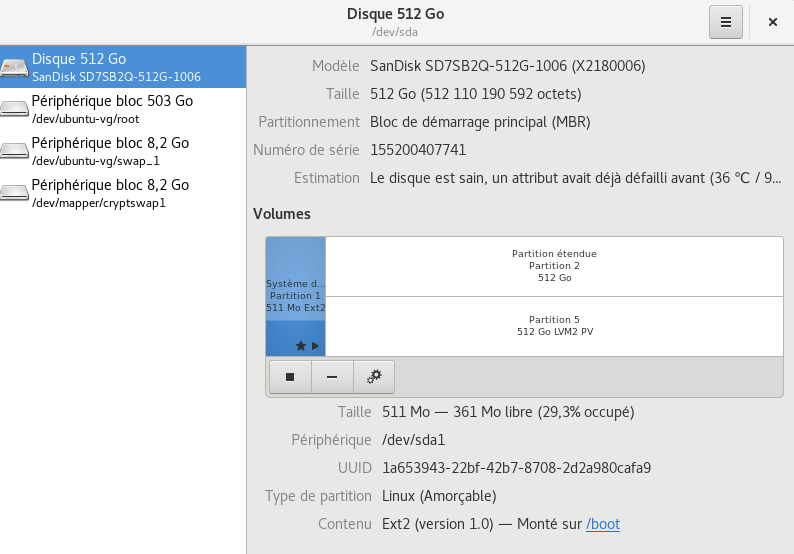
\includegraphics[scale=0.25]{Figures/Selection002}
	\caption{Disques sous GNOME}
	\end{figure}
	\end{center}
	
\end{frame}

\begin{frame}[containsverbatim]
  \frametitle{Sous GNOME 3}
	
	\begin{center}
	\begin{figure}
	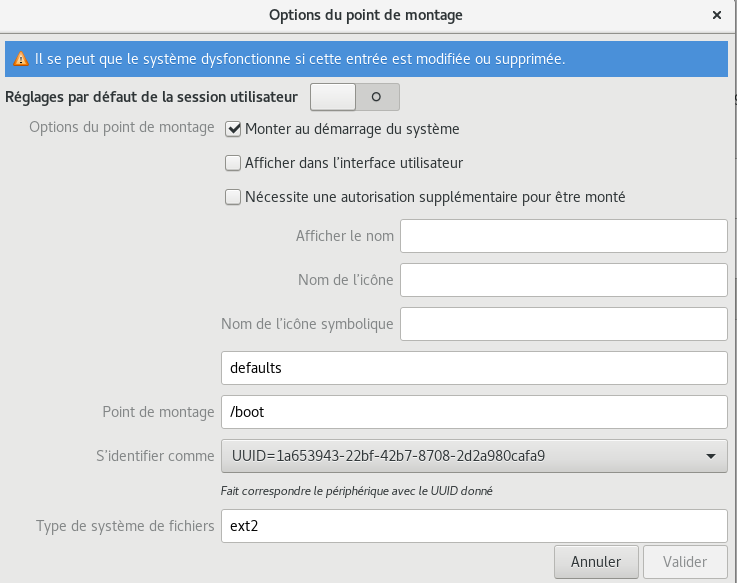
\includegraphics[scale=0.25]{Figures/Selection003}
	\caption{Disques sous GNOME}
	\end{figure}
	\end{center}
	
\end{frame}

\subsection{Ajouter le montage d'un disque au d�marrage}
\begin{frame}[containsverbatim]
  \frametitle{/etc/fstab}

	Comme on a vu pr�cedemment, on utilise l'UUID dans ce fichier de configuration plut�t que le nom de p�riph�rique.

\begin{verbatim}
UUID=c3cc32c0-b4bd-... /boot ext2 defaults 0 2
\end{verbatim}
		
\end{frame}

\begin{frame}[containsverbatim]
  \frametitle{/etc/fstab}

	Attention, au d�marrage, le syst�me risque de se bloquer si le disque est marqu� comme � monter par d�faut
	et qu'il n'est pas pr�sent. Avant d'enlever un disque penser � commenter la ligne (ou la supprimer) avant le 
	red�marrage.

\begin{verbatim}
UUID=c3cc32c0-b4bd-... /boot ext2 defaults 0 2
\end{verbatim}
		
\end{frame}

\begin{frame}[containsverbatim]
  \frametitle{/etc/fstab}
	
	Les arguments sont~:

	\begin{enumerate}
		\item l'identifiant ou le nom du p�riph�rique
		\item le point de montage
		\item le type de la partition
		\item des mots clefs pour changer les propri�t�s du disque
		\item le \emph{dump}, utilis� pour les sauvegardes
		\item le \emph{pass}, pour les v�rifications on d�marrage
	\end{enumerate}
	
\end{frame}

\begin{frame}[containsverbatim]
  \frametitle{/etc/fstab}
	
	Parmi les mots-clefs � conna�tre~:

	\begin{description}
		\item [user, no user] d�finit si un utilisateur (et pas seulement le root) a le droit de monter la partition
		\item [auto,noauto] d�finit si la partition est mont�e automatiquement au d�marrage et en faisant \emph{mount -a}
		\item [atime/noatime] d�finit si le syst�me marque la date de dernier acc�s. Il faut le mettre de pr�f�rence � \emph{noatime} pour les SSD
		\item [rw/ro] montage en lecture/�criture ou lecture seule (read only)
		\item [uid,gid,\dots] permet de sp�cifier les droits des fichiers du disque
	\end{description}
	
\end{frame}

\begin{frame}[containsverbatim]
  \frametitle{/etc/fstab}

	Pour le \emph{dump}, il faut le laisser � 0. 
	
	Pour le \emph{pass}, les valeurs sont � indiquer sont les suivantes~:
	
	\begin{enumerate}
		\item pour la racine
		\item pour les autres partitions Linux
		\item pour le swap et les partitions windows
	\end{enumerate}
	
	Plus d'infos \href{https://doc.ubuntu-fr.org/mount_fstab}{l�}
	
	
\end{frame}

\begin{frame}[containsverbatim]
  \frametitle{/etc/mtab}
	
	
\end{frame}

\section{Les autres r�pertoires}

\subsection{Les devices}

\begin{frame}[containsverbatim]
  \frametitle{Le r�pertoire /dev/}

	Il y a un dicton qui dit que tout dans \GNULinux est fichier.
	
	Ce qui traduit l'existence du r�pertoire \emph{/dev/}. A une entr�e dans ce r�pertoire correspond un mat�riel ou une fonctionnalit� du noyau.
	
	Par exemple avec la commande \emph{sudo blkid} vous pouvez voir les r�pertoires \emph{/dev/} correspondant aux disques.
	
	Un autre exemple est \emph{/dev/urandom} qui contient des donn�es al�atoires g�n�r�es par le noyau.
	
	\begin{verbatim}
dd bs=4M count=1 if=/dev/urandom of=random.txt
	\end{verbatim}

\end{frame}

\begin{frame}[containsverbatim]
  \frametitle{Le r�pertoire /dev/}

	Les fichiers respectent des nomenclatures. Par exemple, \emph{sdX} designe un disque SCSI (historiquement).
	
	\emph{/dev/sdg} d�signe le disque tout entier, \emph{/dev/sdg1} la partition 1 du disque sdg.
	
	Un utilitaire en ligne de commande pour explorer les disques est \emph{fdisk} ou plus r�cent \emph{parted}.
	
	Graphiquement utiliser \emph{gparted}.

\end{frame}

\subsection{Les autres r�pertoires}

\begin{frame}[containsverbatim]
  \frametitle{Les principaux r�pertoire\dots}
	
	\begin{itemize}
		\item /bin, la plupart des programmes en ligne de commande
		\item /dev, pointe vers les p�rph�riques
		\item /etc, Contient les fichiers de configuration du syst�me
		\item /lib, les librairies
		\item /tmp, pour les r�pertoires temporaires
		\item /usr, l� o� s'installe la plupart des programmes
		\item /var, contient les informations partag�e (par exemple site web, logs, \dots)
	\end{itemize}

	La liste compl�te est \href{https://www.dell.com/support/article/fr/fr/frbsdt1/sln152018/the-types-and-definitions-of-ubuntu-linux-partitions-and-directories-explained?lang=en#FileSystem}{l�}.

\end{frame}

\begin{frame}[containsverbatim]
  \frametitle{/bin}

	Dans ce r�pertoire on trouve les binaires c'est-�-dire les programmes ex�cutables.
	
	Vous pouvez �galement trouver des ex�cutables dans les r�pertoires \emph{/usr/share/bin} et \emph{/usr/local/bin}.
	
	La disposition des ex�cutables d�pend de la distribution et du type d'ex�cutables.

\end{frame}

\begin{frame}[containsverbatim]
  \frametitle{/etc}

	Si vous voulez modifier la configuration syst�me, il est probable que vous ayez � intervenir dans ce r�pertoire.
	
	Les fichiers sont presque tous des fichiers texte qu'il suffit d'�diter en tant que super utilisateur.

\end{frame}

\begin{frame}[containsverbatim]
  \frametitle{/lib}

	C'est le r�pertoire dans lequel on trouve les librairies c'est-�-dire des \og~morceaux~\fg de programme qui sont mis dans le pot commun pour plusieurs programmes.

\end{frame}



\begin{frame}[containsverbatim]
  \frametitle{/tmp}

	Dans ce r�pertoire on trouve tous les fichiers qui sont destin�s � avoir une dur�e de vie courte. D'ailleurs sur la plupart des distributions, le r�pertoire est vid� quand le syst�me d�marre.

\end{frame}

\begin{frame}[containsverbatim]
  \frametitle{/usr}

	Dans ce r�pertoire on trouve pas mal de choses. Il y a aussi des ex�cutables des librairies, l'emplacement de tout �a est r�gi par des r�gles d�pendant de la distributions et de l'histoire de \GNULinux. 

	Dans ce r�pertoire on trouve surtout les ex�cutables qui sont lanc�s en mode graphique.

\end{frame}

\begin{frame}[containsverbatim]
  \frametitle{/var}

	Ce r�pertoire est important notamment car vous trouverez par exemple deux r�pertoires tr�s pr�cieux~:
	\begin{itemize}
		\item /var/www, le contenu de votre site web
		\item /var/logs, les fichiers journaux qui stockent les �v�nements qui se produisent sur le poste.
	\end{itemize}

\end{frame}

\begin{frame}[containsverbatim]
  \frametitle{/var}

	La \href{https://www.dell.com/support/article/fr/fr/frbsdt1/sln152018/the-types-and-definitions-of-ubuntu-linux-partitions-and-directories-explained?lang=en}{page} est 
	assez exhaustive.
	
		Elle contient pas d'informations int�ressantes.

\end{frame}

\section{Les formats de partition}

\begin{frame}[containsverbatim]
  \frametitle{Les formats extX}

	Particularit� des syst�mes de fichier
	
	sortie de fdisk -l

\end{frame}

\begin{frame}[containsverbatim]
  \frametitle{Les formats extX}

\begin{verbatim}
file -sL /dev/sd*
\end{verbatim}

\end{frame}

\begin{frame}[containsverbatim]
  \frametitle{Les formats extX}

	\begin{description}
		\item[ext2] c'est le format standard UNIX qui n'est plus au go�t du jour
		\item[ext3] il reprend le format ext2 avec une journalisation
		\item[ext4] il reprend ext3 avec en plus une augmentation de la taille des disques
	\end{description}
	
	A l'heure actuelle, il faut pr�f�rer le format le plus r�cent ext4.
	

\end{frame}

\begin{frame}[containsverbatim]
  \frametitle{Les formats Windows}

	Si vous voulez monter des disques Windows~:

	\begin{description}
		\item[FAT,FAT32] c'est le vieux format qu'on retrouve sur les clefs USB notamment. Il est compatible \Linux, Mac OS et Windows
		\item[NTFS] c'est le \og~nouveau~\fg format de Windows qui est propri�taire
	\end{description}
	
	Avant \Linux ne pouvait �crire que sur des partitions FAT mais maintenant il peut aussi �crire sur des partitions NTFS dans la plupart des distros 
	(mais pas toutes!).
	
\end{frame}

\begin{frame}[containsverbatim]
  \frametitle{Les formats Windows}

	Il y a d'autres types de partitions propos�es~: reiserfs, xfs, zfs, \dots
	
	Il ne se sont pas install�s et/ou sont propri�taires donc ne sont pas lus par toutes les distributions.
	
\end{frame}



\subsection{gparted}
\begin{frame}[containsverbatim]
  \frametitle{gparted}

\end{frame}

\section{Les permissions}

\subsection{permission}

\begin{frame}[containsverbatim]
  \frametitle{les sorties d'un ls}
  
  \begin{verbatim}
  -rw-r--r-- 1 root root 1426 nov.  26  2016 debug
-rw-r--r-- 1 root root 1735 nov.  26  2016 dhclient.conf
drwxr-xr-x 2 root root 4096 nov.   1 12:29 dhclient-enter-hooks.d
drwxr-xr-x 2 root root 4096 nov.   1 12:29 dhclient-exit-hooks.d
  \end{verbatim}
  
  \end{frame}

\begin{frame}[containsverbatim]
  \frametitle{les sorties d'un ls}

Les premiers caract�res sont les droits pour le propri�taire et le groupe attribu� au fichier ou au r�pertoire~:
\begin{description}
	\item[d] directory ou r�pertoire.  
	\item[r] on peut lire le fichier
	\item[w]on peut �crire le fichier
	\item[x] le fichier est ex�cutable ou le r�pertoire peut �tre travers�
\end{description}
  
  si au lieu d'un de ces caract�res est remplac� par un - alors la propri�t� est invers� : si au lieu d'un w on a  -, alors on ne peut pas �crire dans le fichier.
  
  \end{frame}
		
\begin{frame}[containsverbatim]
  \frametitle{Les diff�rents utilisateurs}

On peut voir que le trio rwx est r�p�t� trois fois.

Car il y a trois types d'utilisateurs~:
\begin{enumerate}
	\item le propri�taire du fichier ou \emph{u(ser)}
	\item un membre du groupe auquel est attach� le fichier ou \emph{g(roup)}
	\item tous les autres utilisateurs ou emph{o(thers)}
\end{enumerate}
  
  \end{frame}


\begin{frame}[containsverbatim]
  \frametitle{Dans l'explorateur de fichier}

Avec un clic droit sur le fichier on peut changer avec nautilus ou dolphin, changer les droits~: il suffit de choisir \emph{Propri�t�s} puis \emph{Permissions}.

En ligne de commande vous avez chmod. Il y a plusieurs utilisations de chmod.
  
  \end{frame}

\begin{frame}[containsverbatim]
  \frametitle{Utilisation simple de chmod}

par exemple pour changer les propri�t�s d'un fichier, il faut faire~:
\begin{verbatim}
chmod ug+rwx fichier
\end{verbatim}
  
  cette commande permet de rendre lisible et en �criture \emph{fichier}.
  
  L'inconv�nient est que la syntaxe ne permet de ne changer que par diff�rence les permissions.
  
  \end{frame}



\begin{frame}[containsverbatim]
  \frametitle{Masque}

	Au lieu de modifier les permissions de fa�on relative, elle d�finisse les droits mais sont 
moins intuitifs. A chaque cat�gorie rwx, est assign� un num�ro et la somme d�finie les droits du fichiers.

\begin{description}  
	\item[1] ex�cution
	\item[2] �criture autoris�e
	\item[4] lecture autoris�e 
\end{description}

En combinant les sommes de chacun de ces chiffres on obtient tous les combinaisons de droits.

  \end{frame}

\begin{frame}[containsverbatim]
  \frametitle{Masque}

Ex~: \emph{chmod 754 fichier}
\begin{description}  
	\item[7=] $4+3+1$, tous les droits sont donn�es
	\item[5=] $4+1$, lecture et ex�cution
	\item[4=] $4$, lecture autoris�e 
\end{description}

et ainsi de suite.

  \end{frame}


\begin{frame}[containsverbatim]
  \frametitle{R�cursif}
  
 Pour changer les droits de tout un r�pertoire et ses sous r�pertoires, il suffit de faire
 \emph{chmod 700 -R repertoire} 

Attention, changer les droits des fichiers doit �tre fait de fa�on tr�s prudente car il est diffcile apr�s une erreur de retrouver les droits de tous les fichiers d'une arborescence.

Et parfois le syst�me peut �tre bloqu� pour des probl�mes de droit.

Par exemple, vous bloquerez la mise � jour des fichiers de log si vous en changez les droits.

  \end{frame}

\begin{frame}[containsverbatim]
  \frametitle{Utilisateur et groupe}
 
 il y a deux commandes ~:
 \begin{description}
 	\item[chown pascal fichier] change le propri�taire de fichier pour pascal
 	\item[chown pascal:pascal fichier] change le propri�taire de fichier pour pascal et le groupe pour pascal
 	\item[chgrp pascal fichier] change le propri�taire de fichier pour pascal et le groupe pour pascal
  \end{description}
  
  
  \end{frame}

\section{Utilitaires}
\begin{frame}[containsverbatim]
  \frametitle{Utilitaires}
  
  Il y a quelque utilitaires qui n'ont pas d'�quivalent en mode graphique.
  
  Le premier est \emph{df} qui permet d'avoir la place libre sur les disques.
  
  Il faut le lancer avec l'argument \emph{df -h} pour avoir l'espace en unit�s intelligible.
  
  Il y a aussi la commande \emph{du -ch} qui permet d'avoir l'espace disque pris par des r�pertoires.
  
Sous GNOME, un utilitaire peu efficace qui tente de les remplacer~: \emph{Analyseur d'utilisation de disques}
  
  \end{frame}





\end{document}
\section{R�seau}

\subsection{D�boguer un r�seau}

  \subsection{Je n'ai pas de connexion du tout}
		
	Si vous faites un \emph{ifconfig} et que l'interface r�seau ethernet (enX ou ethX) n'apparait pas\dots
	
	Votre controleur r�seau n'est pas reconnue par \GNULinux. Dans ce cas il faut regarder sur Internet comment l'activer
	pour \GNULinux. Ca peut �tre compliqu�.
	
	G�n�ralement il faut t�l�charger le firmware ou charger le bon module du noyau.
	

		
	Si vous faites un \emph{ifconfig} une adresse internet n'est pas assign�e\dots
	
	Dans ce cas, il est probable que ce soit un cable ou que la box ne joue pas son r�le de DHCP. Le r�seau est indisponible.
	
	Essayer de jouer avec les cables, rebooter votre box, \dots
		

		
	Si vous faites un \emph{ifconfig} une adresse internet n'est assign�e\dots
	
	La box joue son r�le de DHCP. Le r�seau est disponible. Essayer de faire \emph{ping 4.4.4.4}. \emph{4.4.4.4} est un
	serveur de Google qui r�pond au ping sauf cataclysme.
	
	Si vous obtenez une r�ponse alors c'est surement le serveur DNS qui est mal configur� si vous avez 
	un serveur DNS priv� ou vous avez un peu trop jou� avec les r�glages de resolv.conf ou un probl�me
	de pare-feu mal configur� sur la box ou votre routeur.
	
	Si vous n'avez pas de r�ponse au \emph{ping} alors vous n'�tes pas connect� � internet. Dans ce cas
	c'est souvent un probl�me	de pare-feu mal configur� sur la box ou votre routeur.
	
	Autre possibilit� si tout parait au vert mais que vous n'avez pas acc�s au web, v�rifier les r�glages Proxy de votre navigateur.
	



\documentclass{beamer}
\usetheme[compress]{Singapore}
%\useoutertheme{miniframes}

% \documentclass{beamer}
%\usetheme{Warsaw}

% Pour les documents en francais...
	\usepackage[latin1]{inputenc}
	\usepackage[french]{babel}
	\usepackage[french]{varioref}
%\usepackage[T1]{fontenc} 

% Math?matiques
	\usepackage{amsmath}

% Caracteres speciaux suppl?mentaires
	\usepackage{latexsym,amsfonts}

% A documenter
	\usepackage{moreverb}

% Macros pour les paquets
	\usepackage{array}  			% N?cessaires pour les tableaux de la macro Excel.

% Outil suppl?mentaire pour les tableaux
	\usepackage{multirow}
	\usepackage{booktabs}
	\usepackage{xcolor} % alternating row colors in table, incompatible avec certains modules
	\usepackage{longtable}
	\usepackage{colortbl}

% Pour ins?rer des graphiques
	\usepackage{graphicx} 			% Graphique simples
	\usepackage{subfigure}			% Graphiques multiples

% Pour ins?rer des couleurs
	\usepackage{color}

% Rotation des objets et des pages
%	\usepackage{rotating}
%	\usepackage{lscape}

% Pour insrer du code source, LaTeX ou SAS par exemple.
	\usepackage{verbatim}
         \usepackage{moreverb}
	\usepackage{listings}
	\lstset{basicstyle=\ttfamily,
  		showstringspaces=false,
  		commentstyle=\color{red},
  		keywordstyle=\color{blue}
	}
	\usepackage{fancyvrb}

%	\lstset{language=SAS,numbers=left}		% Par dfaut le listing est en SAS

% Pour ins?rer des hyperliens
  \usepackage{hyperref}

% American Psychological Association (for bibliographic references).
	\usepackage{apacite}

% Pour l'utilisation des macros
	\usepackage{xspace}

% Pour l'utilisation de notes en fin de document.
%	\usepackage{endnotes}

% Array
%	\usepackage{multirow}
%	\usepackage{booktabs}

% Rotation
%	\usepackage{rotating}

% En t?tes et pieds de pages
%	\usepackage{fancyhdr}
%	\usepackage{lastpage}


% Page layout

% By LaTeX commands
%\setlength{\oddsidemargin}{0cm}
%\setlength{\textwidth}{16cm}
%\setlength{\textheight}{24cm}
%\setlength{\topmargin}{-1cm}
%\setlength{\marginparsep}{0.2cm}

% fancyheader parameters
%\pagestyle{fancy}

%\fancyfoot[L]{{\small Formation \LaTeX, DEPP}}
%\fancyfoot[c]{}
%\fancyfoot[R]{{\small \thepage/\pageref{LastPage}}}

%\fancyhead[L]{}
%\fancyhead[c]{}
%\fancyhead[R]{}

% Pour ins?rer des dessins de Linux
\newcommand{\LinuxA}{\includegraphics[height=0.5cm]{Graphiques/linux.png}}
\newcommand{\LinuxB}{\includegraphics[height=0.5cm]{Graphiques/linux.png}\xspace}

% Macro pour les petits dessins pour les diff?rents OS.
\newcommand{\Windows}{\emph{Windows}\xspace}
\newcommand{\Mac}{\emph{Mac OS X}\xspace}

\newcommand{\Linux}{\emph{Linux}\xspace}
\newcommand{\linux}{\emph{Linux}\xspace}

\newcommand{\GNULinux}{\emph{GNU/Linux}\xspace}
\newcommand{\gnulinux}{\emph{GNU/Linux}\xspace}

\newcommand{\Fedora}{\emph{Feodra}\xspace}
\newcommand{\Ubuntu}{\emph{Ubuntu}\xspace}


\newcommand{\MikTeX}{MiK\tex\xspace}
\newcommand{\latex}{\LaTeX\xspace}


\newcommand{\df}{\emph{data.frame}\xspace}
\newcommand{\liste}{\emph{list}\xspace}
\newcommand{\cad}{c'est-�-dire\xspace}

% Titre
\title{Introduction � GNU/Linux}
\author{Pascal Bessonneau}
\institute{Starinux}
\date{11/2017}

\subtitle{S�curisation}


\newcommand{\hreff}[2]{\underline{\href{#1}{#2}\xspace}}

\begin{document}

\begin{frame}
	\maketitle
\end{frame}

\begin{frame}
	\tableofcontents
\end{frame}

% Begin document %%%%%%%%%%%%%%%%%%%%%%%%%%%%%%%%%%%%%%%%%%%%%%%%%%%%%%%%%%%%%%%%%%%%%%%%%%%%%%%%%%

\section{S�curisation}

\subsection{Super utilisateur et compte ROOT}

\begin{frame}[containsverbatim]
  \frametitle{Compte ROOT}
	
	�tre \emph{root} permet de tout faire sur un poste \gnulinux. C'est le super utilisateur qui permet 
	notamment d'�diter les fichiers syst�mes, arr�ter/d�marrer des services, \dots
	
	Mais il ne faut pas utiliser le compte \emph{root}. En effet on peux supprimer, alt�rer des fichiers syst�mes ou d'autres utilisateurs.
	
	Et si vous le pouvez, surfer sur le web ou lancer des programmes vous expose consid�rablement car un malware peux de profondes modifications
	sur votre ordinateur.
			
\end{frame}

\begin{frame}[containsverbatim]
  \frametitle{Compte ROOT}

		C'est pour cette raison que le compte root doit absolument �tre d�sactiv� sur un poste convenablement s�curis�. C'est le cas par d�faut
		sur les distributions modernes. 
		
		Cette d�sactivation est visible dans le fichier \emph{/etc/passwd} car comme interpr�teur de fichier il doit y avoir \emph{/bin/false}.
		
		\emph{false} est un programme qui �choue lorsqu'on le lance.
			
\end{frame}

\begin{frame}[containsverbatim]
  \frametitle{sudo}

		Comme il n'y a pas de compte \emph{root} et qu'il faut quand m�me pouvoir modifier des fichiers syst�mes, lancer/d�marrer des services, \dots
		il existe la possibilit� d'utiliser l'utilitaire \emph{sudo}.
		
		Les administrateurs (et non le commun des mortels) doit avoir un acc�s � \emph{sudo}. Cela est possible car les administrateurs appartiennent
		au groupe \emph{sudo} (ou \emph{wheel}).
		
		Lorsque vous tapez une commande pr�c�d�e par \emph{sudo} alors cette commande est ex�cut�e en tant que \emph{root} apr�s vous �tre authentifi� 
		avec votre mot de passe. Le mot de passe n'est pas redemand� pendant quelques minutes apr�s une premi�re utilisation de sudo.
		
		Attention, vous pouvez tout casser avec une commande sudo comme si vous �tiez \emph{root}.
				
\end{frame}


\begin{frame}[containsverbatim]
  \frametitle{sudo}

		La diff�rence avec un compte \emph{root} est que le fait d'�tre \emph{root} est transitoire. Ce qui permet de se prot�ger de 
		beaucoup de malwares.
		
		Le nombre de personnes pouvant �tre \emph{sudoers} doit �tre limit� au maximum. D'autant plus que la mise � jour des paquets non critiques
		est possible sur les derni�res distributions par des administrateurs et non par le super utilisateur.
		
		
\end{frame}

\begin{frame}[containsverbatim]
  \frametitle{sudo}

	Enfin il est possible de limiter les commandes que peuvent lancer les \emph{sudoers}. Ceci est possible en �ditant le fichier de configuration de \emph{sudo}
	avec la commande \emph{visudo}.
	
	Par exemple on peut ajouter paul qui a besoin de lancer/relancer apache car il est webmaster. Il suffit alors de rajouter~:
\begin{verbatim}
paul	ALL = /usr/bin/apachectl
\end{verbatim}

	Et il ne faut pas l'ajouter aux utilisateurs sudo. 
	
	Plus d'information sur ces modifications sont disponibles \href{https://doc.ubuntu-fr.org/sudoers}{l�}.
		
\end{frame}


\section{Rappels r�seaux}


\begin{frame}[containsverbatim]
  \frametitle{Protocoles r�seaux}

	On s'int�ressera principalement � trois protocoles~: TCP, UDP et ICMP.
	
	Le protocole TCP est le plus utilis�. Il est utilis� quand une connexion stable et qui n�cessite l'envoi et la r�ception de paquets dans un ordre d�fini.
	
	Le protcole UDP est moins utilis�. Il sert souvent � envoyer des messages o� l'aspect transactionnelle est moins importante comme la vid�o sur le LAN. Il ne garantit
	ni que les donn�es arrivent dans l'autre ni que les deux ordinateurs ont �tabli une connexion.
	
	Le protocole ICMP est un protocole dont on peux se passer mais qui permet d'envoyer des messages sur le r�seau~: saturation du r�seau, �cho, \dots Il n'est pas associ�
	� un port particulier contrairement � TCP et UDP.
		
\end{frame}

\begin{frame}[containsverbatim]
  \frametitle{Protocoles r�seaux}

	Quand vous voulez ouvrir un port pour SSH, votre site web ou une autre application il s'agit souvent de TCP. Quelques applications comme la communication
	sur internet (genre Skype) peuvent demander d'ouvrir un port UDP.
	
	Le protocole ICMP doit �tre accessible par exemple sur des op�rateurs de serveurs tels qu'OVH qui utilisent ce protocole pour v�rifier que la machine 
	est bien \og~Up and running~\fg.
		
\end{frame}


\begin{frame}[containsverbatim]
  \frametitle{Protocoles r�seaux}

	Par d�faut quand une application n'�coute pas sur le port, le port est ferm�. Si une application l'utilise et peut �tablir une connexion dans le sens
	internet vers votre ordinateur, le port est ouvert. Si c'est dans l'autre sens le port est ferm�~: c'est votre ordinateur qui initiera la connexion
	dans le sens votre ordinateur vers internet. 
	
	Un pare-feu permet de prot�ger votre ordinateur en masquant des ports ouverts qui ne devraient pas �tre visibles depuis l'ext�rieur (imprimante 631,
	ssh 22, \dots). Les ports sont alors masqu�s~: votre ordinateur ne renvoie pas un message port ferm� ce qui ne trahi pas sa pr�sence et emp�che la
	connexion depuis l'ext�rieur.
		
\end{frame}

\section{Pare-feu}

\begin{frame}[containsverbatim]
  \frametitle{arno-iptables-firewall}

	C'est un petit pare-feu disponible sous Debian/Ubuntu.
	
	A partir de quelques questions, il met en place un pare-feu tout � fait performant et s�curitaire.
	
	Apr�s installation, les r�glages suppl�mentaires sont situ�s dans le fichier \emph{/etc/default/arno-iptables-firewall} et 
	\emph{/etc/arno-iptables-firewall/firewall.conf}.
	
	Vous trouverez un tutoriel \href{https://www.unixmen.com/install-configure-arno-iptables-ubuntu-14-04-lts/}{l�}.
		
\end{frame}

\begin{frame}[containsverbatim]
  \frametitle{FirewallID}

	La documentation pour FirewallID est disponible sur les sites suivants~:
	\begin{itemize}
		\item \href{https://doc.fedora-fr.org/wiki/Parefeu_-_firewall_-_FirewallD}{l�}
		\item \href{https://packages.debian.org/sid/main/firewalld}{l�}
		\item  \href{https://packages.debian.org/fr/source/sid/firewalld}{l�}
		\item \href{http://www.firewalld.org/}{l�}
	\end{itemize}
	
\end{frame}

\begin{frame}[containsverbatim]
  \frametitle{V�rifier que la pare-feu fonctionne}

	Pour v�rifier que le pare-feu fonctionne vous pouvez utiliser une autre machine de votre r�seau sous Linux.
	Pour cela (installer et) lancer la commande~:
\begin{verbatim}
nmap -sT <ip de la machine � tester>
\end{verbatim}
	
	Si vous avez distingu� un r�seau interne et un r�seau externe les tests sont plus difficiles � r�aliser.
	
\end{frame}


\begin{frame}[containsverbatim]
  \frametitle{V�rifier que la pare-feu fonctionne}

	De fa�on g�n�rale pour v�rifier quels ports sont visibles de l'ext�rieur, vous pouvez utiliser le 
	site \href{https://www.grc.com/shieldsup}{Shields Up !}.
	
\end{frame}

\end{document}
\documentclass{beamer}
\usetheme[compress]{Singapore}
%\useoutertheme{miniframes}

% \documentclass{beamer}
%\usetheme{Warsaw}

% Pour les documents en francais...
	\usepackage[latin1]{inputenc}
	\usepackage[french]{babel}
	\usepackage[french]{varioref}
%\usepackage[T1]{fontenc} 

% Math?matiques
	\usepackage{amsmath}

% Caracteres speciaux suppl?mentaires
	\usepackage{latexsym,amsfonts}

% A documenter
	\usepackage{moreverb}

% Macros pour les paquets
	\usepackage{array}  			% N?cessaires pour les tableaux de la macro Excel.

% Outil suppl?mentaire pour les tableaux
	\usepackage{multirow}
	\usepackage{booktabs}
	\usepackage{xcolor} % alternating row colors in table, incompatible avec certains modules
	\usepackage{longtable}
	\usepackage{colortbl}

% Pour ins?rer des graphiques
	\usepackage{graphicx} 			% Graphique simples
	\usepackage{subfigure}			% Graphiques multiples

% Pour ins?rer des couleurs
	\usepackage{color}

% Rotation des objets et des pages
%	\usepackage{rotating}
%	\usepackage{lscape}

% Pour insrer du code source, LaTeX ou SAS par exemple.
	\usepackage{verbatim}
         \usepackage{moreverb}
	\usepackage{listings}
	\lstset{basicstyle=\ttfamily,
  		showstringspaces=false,
  		commentstyle=\color{red},
  		keywordstyle=\color{blue}
	}
	\usepackage{fancyvrb}

%	\lstset{language=SAS,numbers=left}		% Par dfaut le listing est en SAS

% Pour ins?rer des hyperliens
  \usepackage{hyperref}

% American Psychological Association (for bibliographic references).
	\usepackage{apacite}

% Pour l'utilisation des macros
	\usepackage{xspace}

% Pour l'utilisation de notes en fin de document.
%	\usepackage{endnotes}

% Array
%	\usepackage{multirow}
%	\usepackage{booktabs}

% Rotation
%	\usepackage{rotating}

% En t?tes et pieds de pages
%	\usepackage{fancyhdr}
%	\usepackage{lastpage}


% Page layout

% By LaTeX commands
%\setlength{\oddsidemargin}{0cm}
%\setlength{\textwidth}{16cm}
%\setlength{\textheight}{24cm}
%\setlength{\topmargin}{-1cm}
%\setlength{\marginparsep}{0.2cm}

% fancyheader parameters
%\pagestyle{fancy}

%\fancyfoot[L]{{\small Formation \LaTeX, DEPP}}
%\fancyfoot[c]{}
%\fancyfoot[R]{{\small \thepage/\pageref{LastPage}}}

%\fancyhead[L]{}
%\fancyhead[c]{}
%\fancyhead[R]{}

% Pour ins?rer des dessins de Linux
\newcommand{\LinuxA}{\includegraphics[height=0.5cm]{Graphiques/linux.png}}
\newcommand{\LinuxB}{\includegraphics[height=0.5cm]{Graphiques/linux.png}\xspace}

% Macro pour les petits dessins pour les diff?rents OS.
\newcommand{\Windows}{\emph{Windows}\xspace}
\newcommand{\Mac}{\emph{Mac OS X}\xspace}

\newcommand{\Linux}{\emph{Linux}\xspace}
\newcommand{\linux}{\emph{Linux}\xspace}

\newcommand{\GNULinux}{\emph{GNU/Linux}\xspace}
\newcommand{\gnulinux}{\emph{GNU/Linux}\xspace}

\newcommand{\Fedora}{\emph{Feodra}\xspace}
\newcommand{\Ubuntu}{\emph{Ubuntu}\xspace}


\newcommand{\MikTeX}{MiK\tex\xspace}
\newcommand{\latex}{\LaTeX\xspace}


\newcommand{\df}{\emph{data.frame}\xspace}
\newcommand{\liste}{\emph{list}\xspace}
\newcommand{\cad}{c'est-�-dire\xspace}

% Titre
\title{Introduction � GNU/Linux}
\author{Pascal Bessonneau}
\institute{Starinux}
\date{11/2017}

\subtitle{Sauvetage}


\newcommand{\hreff}[2]{\underline{\href{#1}{#2}\xspace}}

\begin{document}

\begin{frame}
	\maketitle
\end{frame}

\begin{frame}
	\tableofcontents
\end{frame}

% Begin document %%%%%%%%%%%%%%%%%%%%%%%%%%%%%%%%%%%%%%%%%%%%%%%%%%%%%%%%%%%%%%%%%%%%%%%%%%%%%%%%%%

\section{R�paration}

\begin{frame}[containsverbatim]
  \frametitle{Utilitaire Live CDs}
 
 Pour la plupart des distributions, il y a des live CDs qui vont vous permettre en mode graphique ou en ligne de commande sauvez votre installation.
 
 Il y a m�me des des distributions d�di�es comme \href{http://distrowatch.com/search.php?category=Data+Rescue}{ici}.
 
 Attention la liste contient aussi des distributions de \emph{forensics} pour �tudier un disque apr�s une intrusion (Kali, Backbox).
 
  
  \end{frame}

\begin{frame}[containsverbatim]
  \frametitle{Montage}
 
 Le type de probl�me fr�quent est d'alt�rer /etc/fstab et �a emp�che le syst�me de booter.
 
 Il suffit d'appliquer ce que vous avez appris. 
 
 Il faut identifier votre disque avec la commande \emph{sudo blkid} et/ou \emph{fdisk -l}
 
 
  \end{frame}

\begin{frame}[containsverbatim]
  \frametitle{Montage}

 
 \begin{verbatim}
 sudo mkdir /media/crash
 sudo mount /dev/sdX /media/crash
 sudo nano /media/crash/etc/fstab
 \end{verbatim}
  
  
  \end{frame}

\begin{frame}[containsverbatim]
  \frametitle{Corruption d'un disque}

 Sauf tr�s gros probl�me, vous pouvez lors du d�marage acc�der � la console pour r�parer une parititon d�fecteuse.
 
 Mais si vous voulez corriger une partition d�fectueuse vous pouvez le faire avec la commande~:
 \begin{verbatim}
 sudo e2fsck /dev/sdX
 \end{verbatim}
 
 \textcolor{red}{Attention !!! la partition ne doit pas �tre mont�e pour le faire} 
 
  \end{frame}
 
 \begin{frame}[containsverbatim]
  \frametitle{Corruption d'un disque}

\emph{e2fsck} d�tecte le type de partition et tente de r�parer le disque.

  Si \emph{e2fsck} ne d�tecte pas le type de partition l�, soit vous vous �tes tromp� en sp�cifiant la partition soit elle est tr�s abim�e et sera �ventuellement r�cup�rable en for�ant 
  
  \emph{e2fsck.ext4},  \emph{e2fsck.ext3}, \dots
  
  La r�cup�ration des disques Windows (fat, ntfs) est un probl�me sous Linux car elle ne marche pas tr�s bien et vous demande souvent de faire la r�paration sous\dots Windows.
  
  \end{frame}


\begin{frame}[containsverbatim]
  \frametitle{Grub}

Si l'ordinateur ne d�marre pas du tout hors mat�riel c'est potentiellement grub qui pose probl�me. Dans ce il faut r�parer grub.

La solution c'est le chroot. Cet utilitaire va faire croire au syst�me que la racine est diff�rente et vous pourrez faire fonctionner comme si vous aviez booter sur le syt�me alt�r�. 
 
C'est-�-dire que si vous voulez acc�der � /mnt/t1/boot/grub.cfg, vous le ferez en acc�dant directement par /boot/grub.cfg une fois chroot�.  
  
  \end{frame}

\begin{frame}[containsverbatim]
  \frametitle{Grub}

Il faut monter la partition par exemple dans le r�pertoire /mnt/t1 puis~:
\begin{verbatim}
mount /dev/sda1 /mnt/t1
mount --bind /run  /mnt/t1/run
mount --bind /dev /mnt/t1/dev
mount --bind /dev/pts /mnt/t1/dev/pts
mount -t proc /proc /mnt/t1/proc
mount -t sysfs /sys /mnt/t1/system/sys
chroot /mnt/t1 /bin/bash
\end{verbatim} 
  
  \end{frame}

\begin{frame}[containsverbatim]
  \frametitle{Grub}

une fois chroot� il suffira d'un~:
\begin{verbatim}
sudo update-grub
\end{verbatim} 
  
  \end{frame}




\end{document}
\end{document}
